\def\retinafocusresults{
    Một đặc điểm của mô hình RetinaFocus là có nhiều cấu hình có thể cài đặt để triển khai mô hình như cấu hình lựa chọn bản đồ đặc trưng\index{bản đồ đặc trưng} của FPN cho nhánh tập trung đối tượng\index{nhánh tập trung đối tượng}, cấu hình tuỳ chỉnh kích thước ảnh trong quá trình dự đoán \dots
    Vì vậy, ta cần so sánh và lựa chọn cấu hình tối ưu nhất, cân đối giữa thời gian thực hiện quá trình dự đoán và độ chính xác của mô hình.
    Để so sánh một cách toàn diện nhất, ta sẽ sử dụng cả hai bộ dữ liệu WIDER FACE thông thường và bộ dữ liệu WIDER FACE kích thước lớn.

    \noindent
    Để đánh giá một cách khách quan sự đánh đối giữa tốc độ và độ chính xác của các mô hình, ta sử dụng chỉ số Average Precision (AP) để đánh giá độ chính xác của mô hình nhận diện khuôn mặt và chỉ số thời gian dự đoán của mô hình trên các bộ dữ liệu kiểm thử (đơn vị là giây).

    \noindent
    Các thí nghiệm dự đoán trong phần này được thực hiện trên một GPU NVIDIA GeForce RTX 2080 Ti.

    \subsubsection*{Thí nghiệm so sánh các cấu hình sử dụng bản đồ đặc trưng\index{bản đồ đặc trưng} khác nhau của FPN làm đầu vào cho nhánh tập trung đối tượng}
    Trong thí nghiệm này, với mỗi cấu hình, chúng tôi sử dụng các bản đồ đặc trưng\index{bản đồ đặc trưng} khác nhau của FPN làm đầu vào cho nhánh tập trung đối tượng\index{nhánh tập trung đối tượng}. \\
    Trong đó, lần lượt các cấu hình sử dụng bản đồ đặc trưng\index{bản đồ đặc trưng} ${C}_{3}, {C}_{4}, {C}_{5}, {P}_{3}, {P}_{4}, {P}_{5}$ được ký hiệu là \textit{using feature maps C3}, \textit{using feature maps C4}, \textit{using feature maps C5}, \textit{using feature maps P3}, \textit{using feature maps P4}, \textit{using feature maps P5} trong các biểu đồ.
    Trong các cấu hình trên, các cặp bản đồ đặc trưng\index{bản đồ đặc trưng} ${C}_{3}$ và ${P}_{3}$, ${C}_{4}$ và ${P}_{4}$, ${C}_{5}$ và ${P}_{5}$ là các cặp bản đồ đặc trưng\index{bản đồ đặc trưng} có cùng kích thước. \\
    Tuy nhiên, mỗi bản đồ đặc trưng\index{bản đồ đặc trưng} khác nhau trong cặp chứa thông tin khác nhau về khuôn mặt dẫn đến số lượng và kích thước của các vùng mà nhánh tập trung đối tượng\index{nhánh tập trung đối tượng} xác định cần phải zoom vào cũng khác nhau.
    Từ đó dẫn đến thời gian thực hiện toàn bộ quá trình dự đoán trên cả bộ dữ liệu là khác nhau. \\
    Trong thí nghiệm này, tất cả các cấu hình sử dụng chung một cấu hình tuỳ chỉnh kích thước ảnh trong quá trình dự đoán mô phỏng lại chiến lược Image Pyramids của RetinaFace.

    \begin{figure}[H]
        \centering
        \subfigure[]{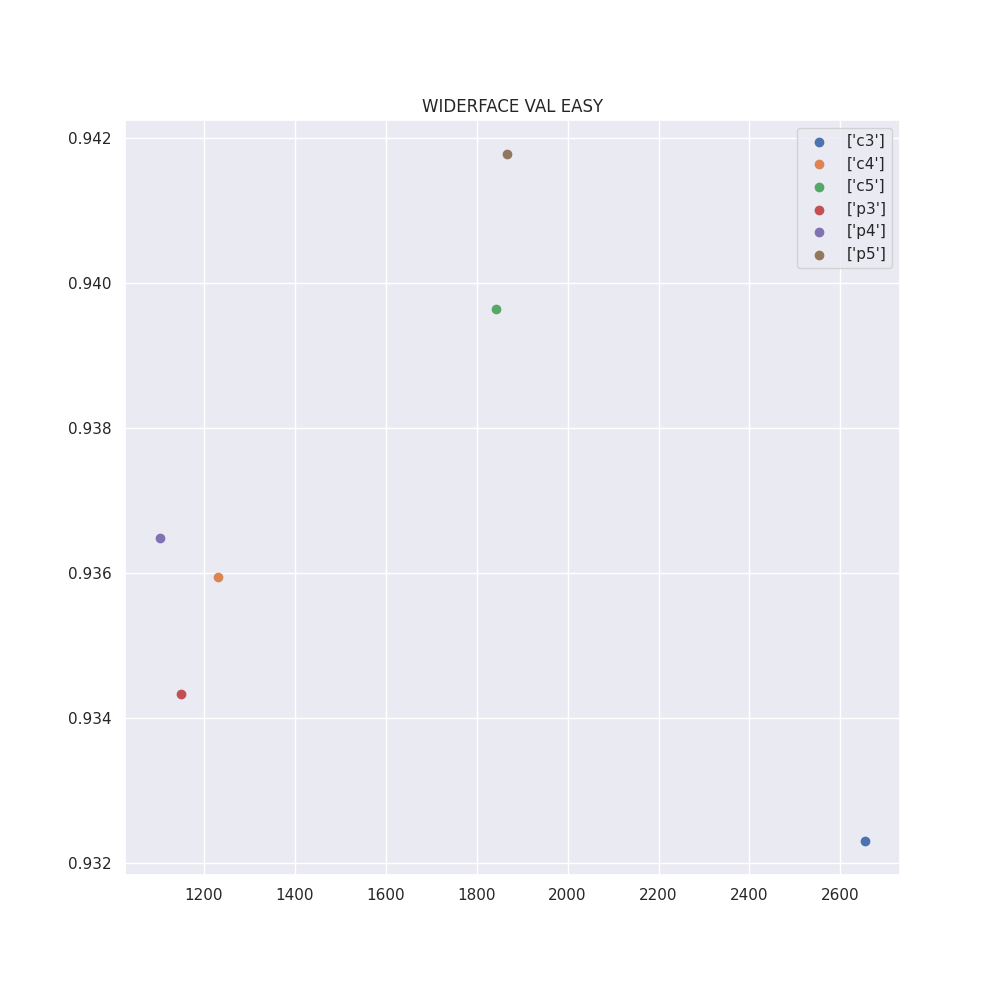
\includegraphics[width=7.3cm]{images/retinafocus_widerface_val_easy_fpn}} 
        \subfigure[]{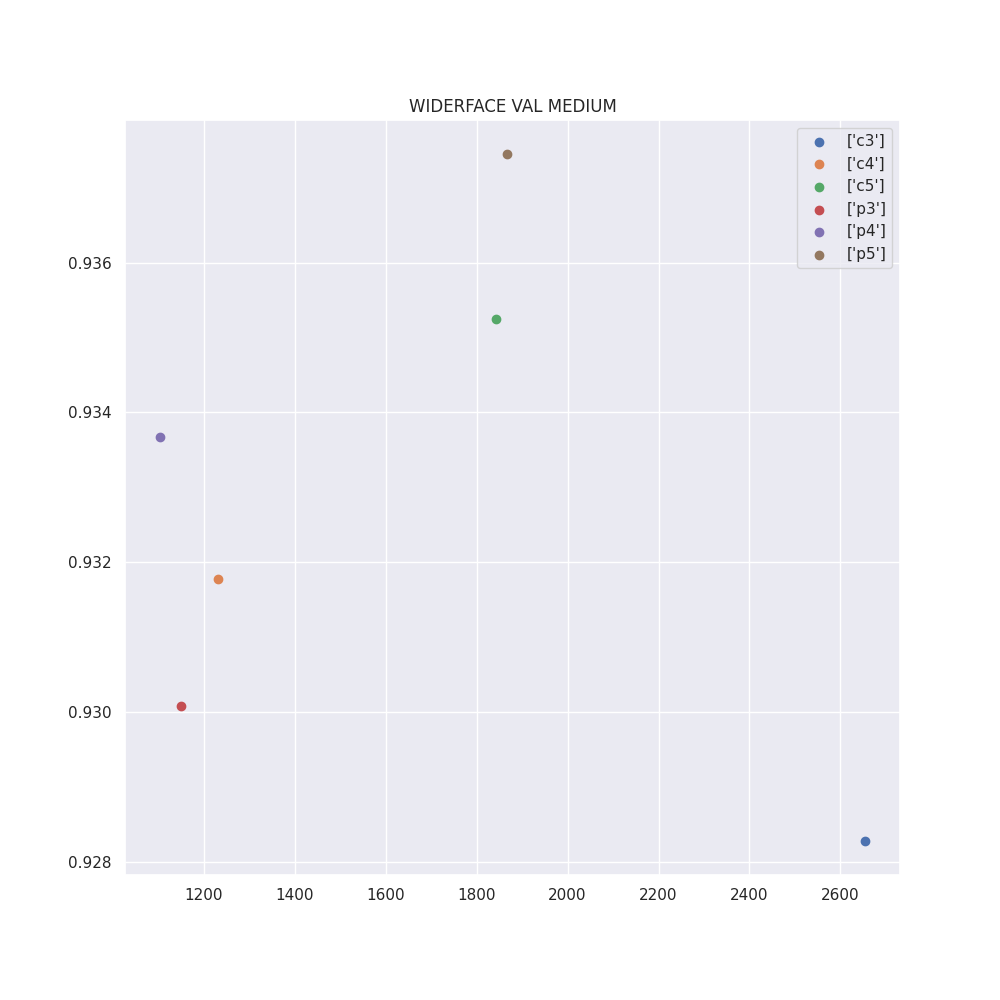
\includegraphics[width=7.3cm]{images/retinafocus_widerface_val_medium_fpn}} 
        \subfigure[]{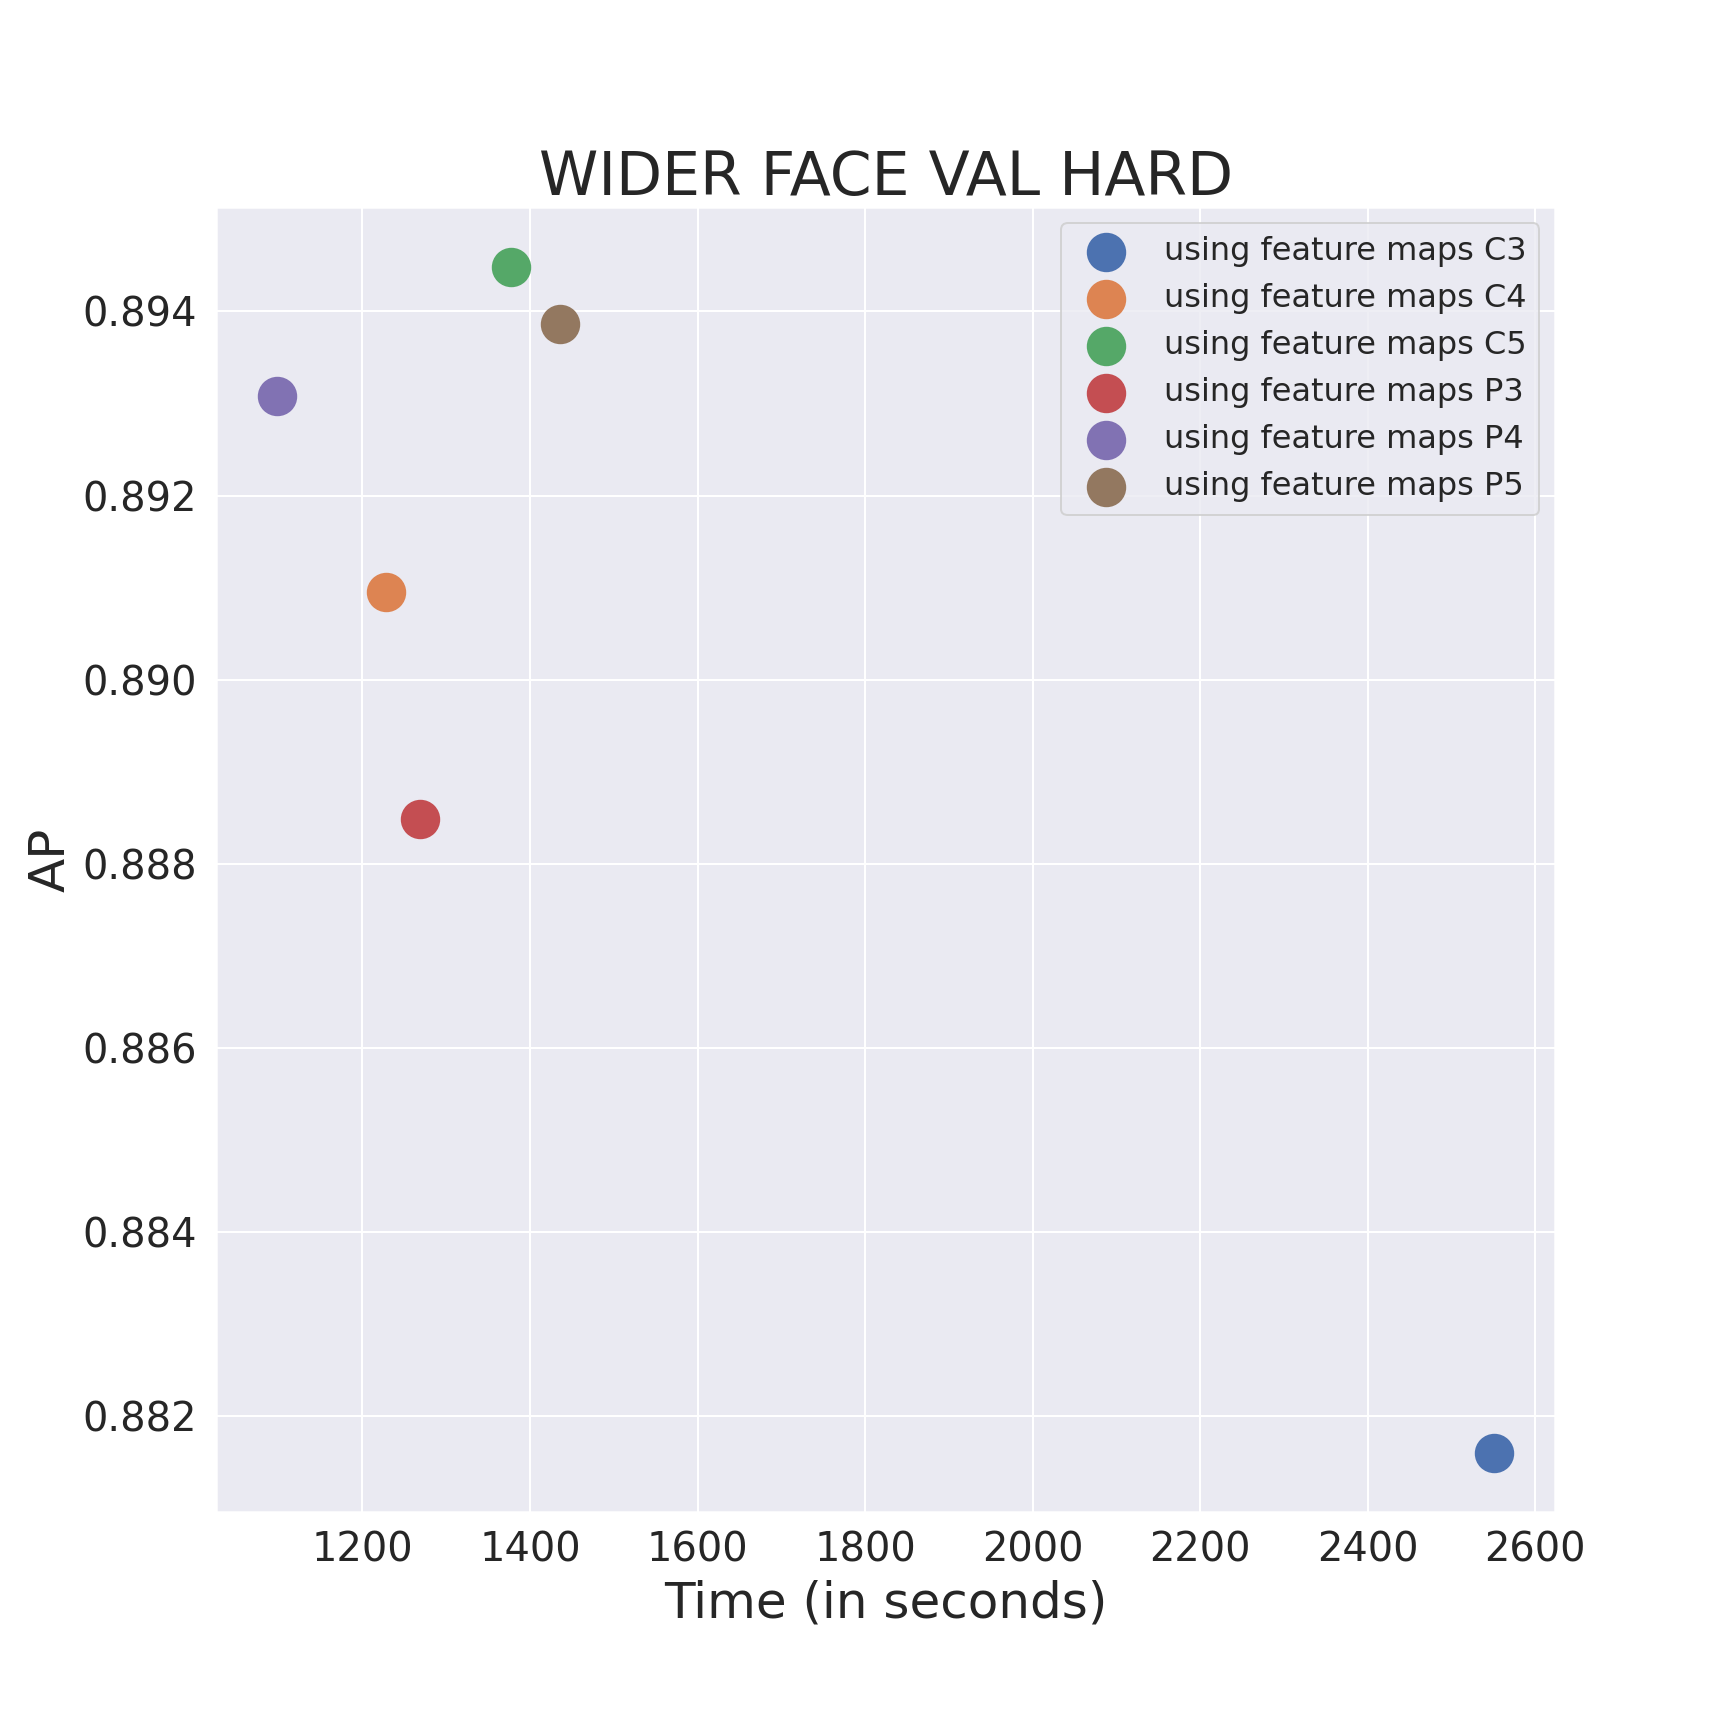
\includegraphics[width=7.3cm]{images/retinafocus_widerface_val_hard_fpn}} 
        \caption{Kết quả so sánh các cấu hình sử dụng các bản đồ đặc trưng\index{bản đồ đặc trưng} của FPN làm đầu vào cho nhánh tập trung đối tượng\index{nhánh tập trung đối tượng} trên ba bộ dữ liệu WIDER FACE val easy (a), medium (b) và hard (c)}
        \label{fig:retinafocus_widerface_val_fpn}
    \end{figure}

    \noindent
    Cụ thể, mô hình RetinaFocus sẽ thực hiện vòng lặp dự đoán năm lần, trong đó: \\
    - Vòng lặp đầu tiên sẽ tuỳ chỉnh kích thước ảnh đầu vào của mô hình nằm trong khoảng từ 500 điểm ảnh\index{điểm ảnh} đến 750 điểm ảnh\index{điểm ảnh}. \\
    - Vòng lặp thứ hai sẽ tuỳ chỉnh kích thước ảnh đầu vào của mô hình tương đương với kích thước ảnh gốc ban đầu nằm trong khoảng từ 800 điểm ảnh\index{điểm ảnh} đến 1200 điểm ảnh\index{điểm ảnh}. \\
    - Vòng lặp thứ ba sẽ tuỳ chỉnh kích thước ảnh đầu vào của mô hình tương đương với kích thước ảnh gốc ban đầu nằm trong khoảng từ 1100 điểm ảnh\index{điểm ảnh} đến 1650 điểm ảnh\index{điểm ảnh}. \\
    - Vòng lặp thứ tư sẽ tuỳ chỉnh kích thước ảnh đầu vào của mô hình tương đương với kích thước ảnh gốc ban đầu nằm trong khoảng từ 1400 điểm ảnh\index{điểm ảnh} đến 2100 điểm ảnh\index{điểm ảnh}. \\
    - Vòng lặp cuối cùng sẽ tuỳ chỉnh kích thước ảnh đầu vào của mô hình tương đương với kích thước ảnh gốc ban đầu nằm trong khoảng từ 1700 điểm ảnh\index{điểm ảnh} đến 2550 điểm ảnh\index{điểm ảnh}.

    \noindent
    Đối với bộ WIDER FACE thông thường, hai cấu hình đạt độ chính xác cao nhất là cấu hình sử dụng bản đồ đặc trưng\index{bản đồ đặc trưng} ${P}_{5}$ và cấu hình sử dụng bản đồ đặc trưng\index{bản đồ đặc trưng} ${C}_{5}$ cho nhánh tập trung đối tượng\index{nhánh tập trung đối tượng} với thời gian thực hiện toàn bộ quá trình dự đoán trên cả bộ dữ liệu lần lượt là 1436 và 1377 giây.
    Trong khi cấu hình sử dụng bản đồ đặc trưng\index{bản đồ đặc trưng} ${P}_{5}$ cho kết quả tốt hơn trên bộ WIDER FACE val easy và medium thì cấu hình sử dụng bản đồ đặc trưng\index{bản đồ đặc trưng} ${C}_{5}$ cho kết quả tốt hơn trên bộ WIDER FACE val hard.
    Các cấu hình khác như ${P}_{4}$, ${P}_{3}$ và ${C}_{4}$ có thời gian thực hiện toàn bộ quá trình dự đoán nhanh hơn nhưng độ chính xác không tốt.
    Đặc biệt là cấu hình ${C}_{3}$ vừa có thời gian thực hiện toàn bộ quá trình dự đoán chậm vừa đạt độ chính xác thấp.

    \begin{figure}[H]
        \centering
        \subfigure[]{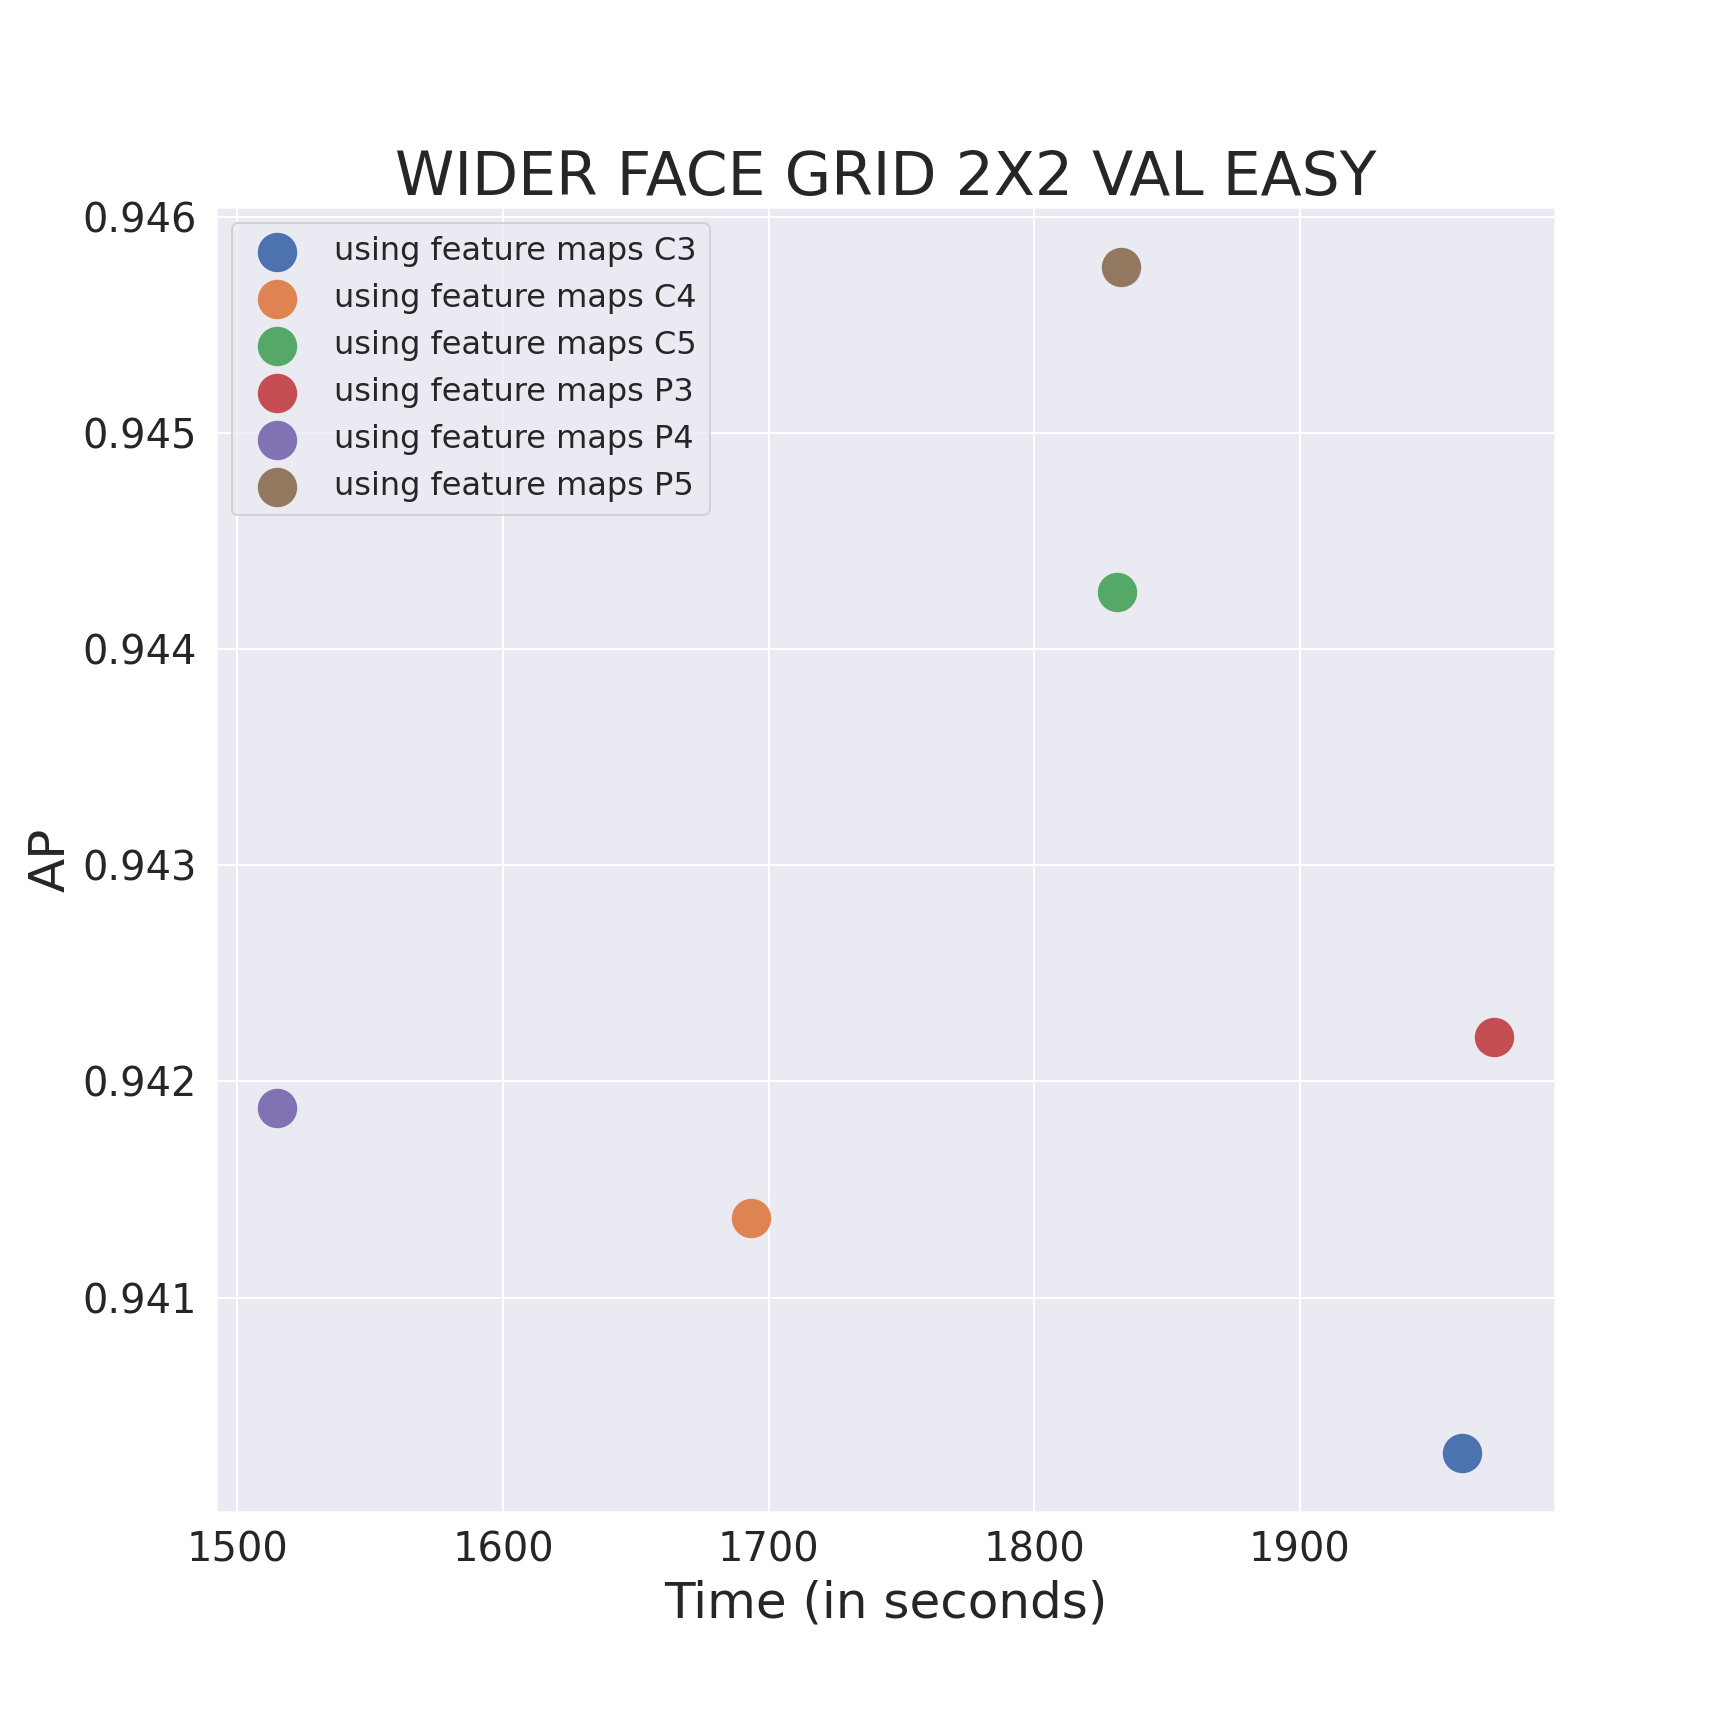
\includegraphics[width=7.3cm]{images/retinafocus_widerface_2k_val_easy_fpn}} 
        \subfigure[]{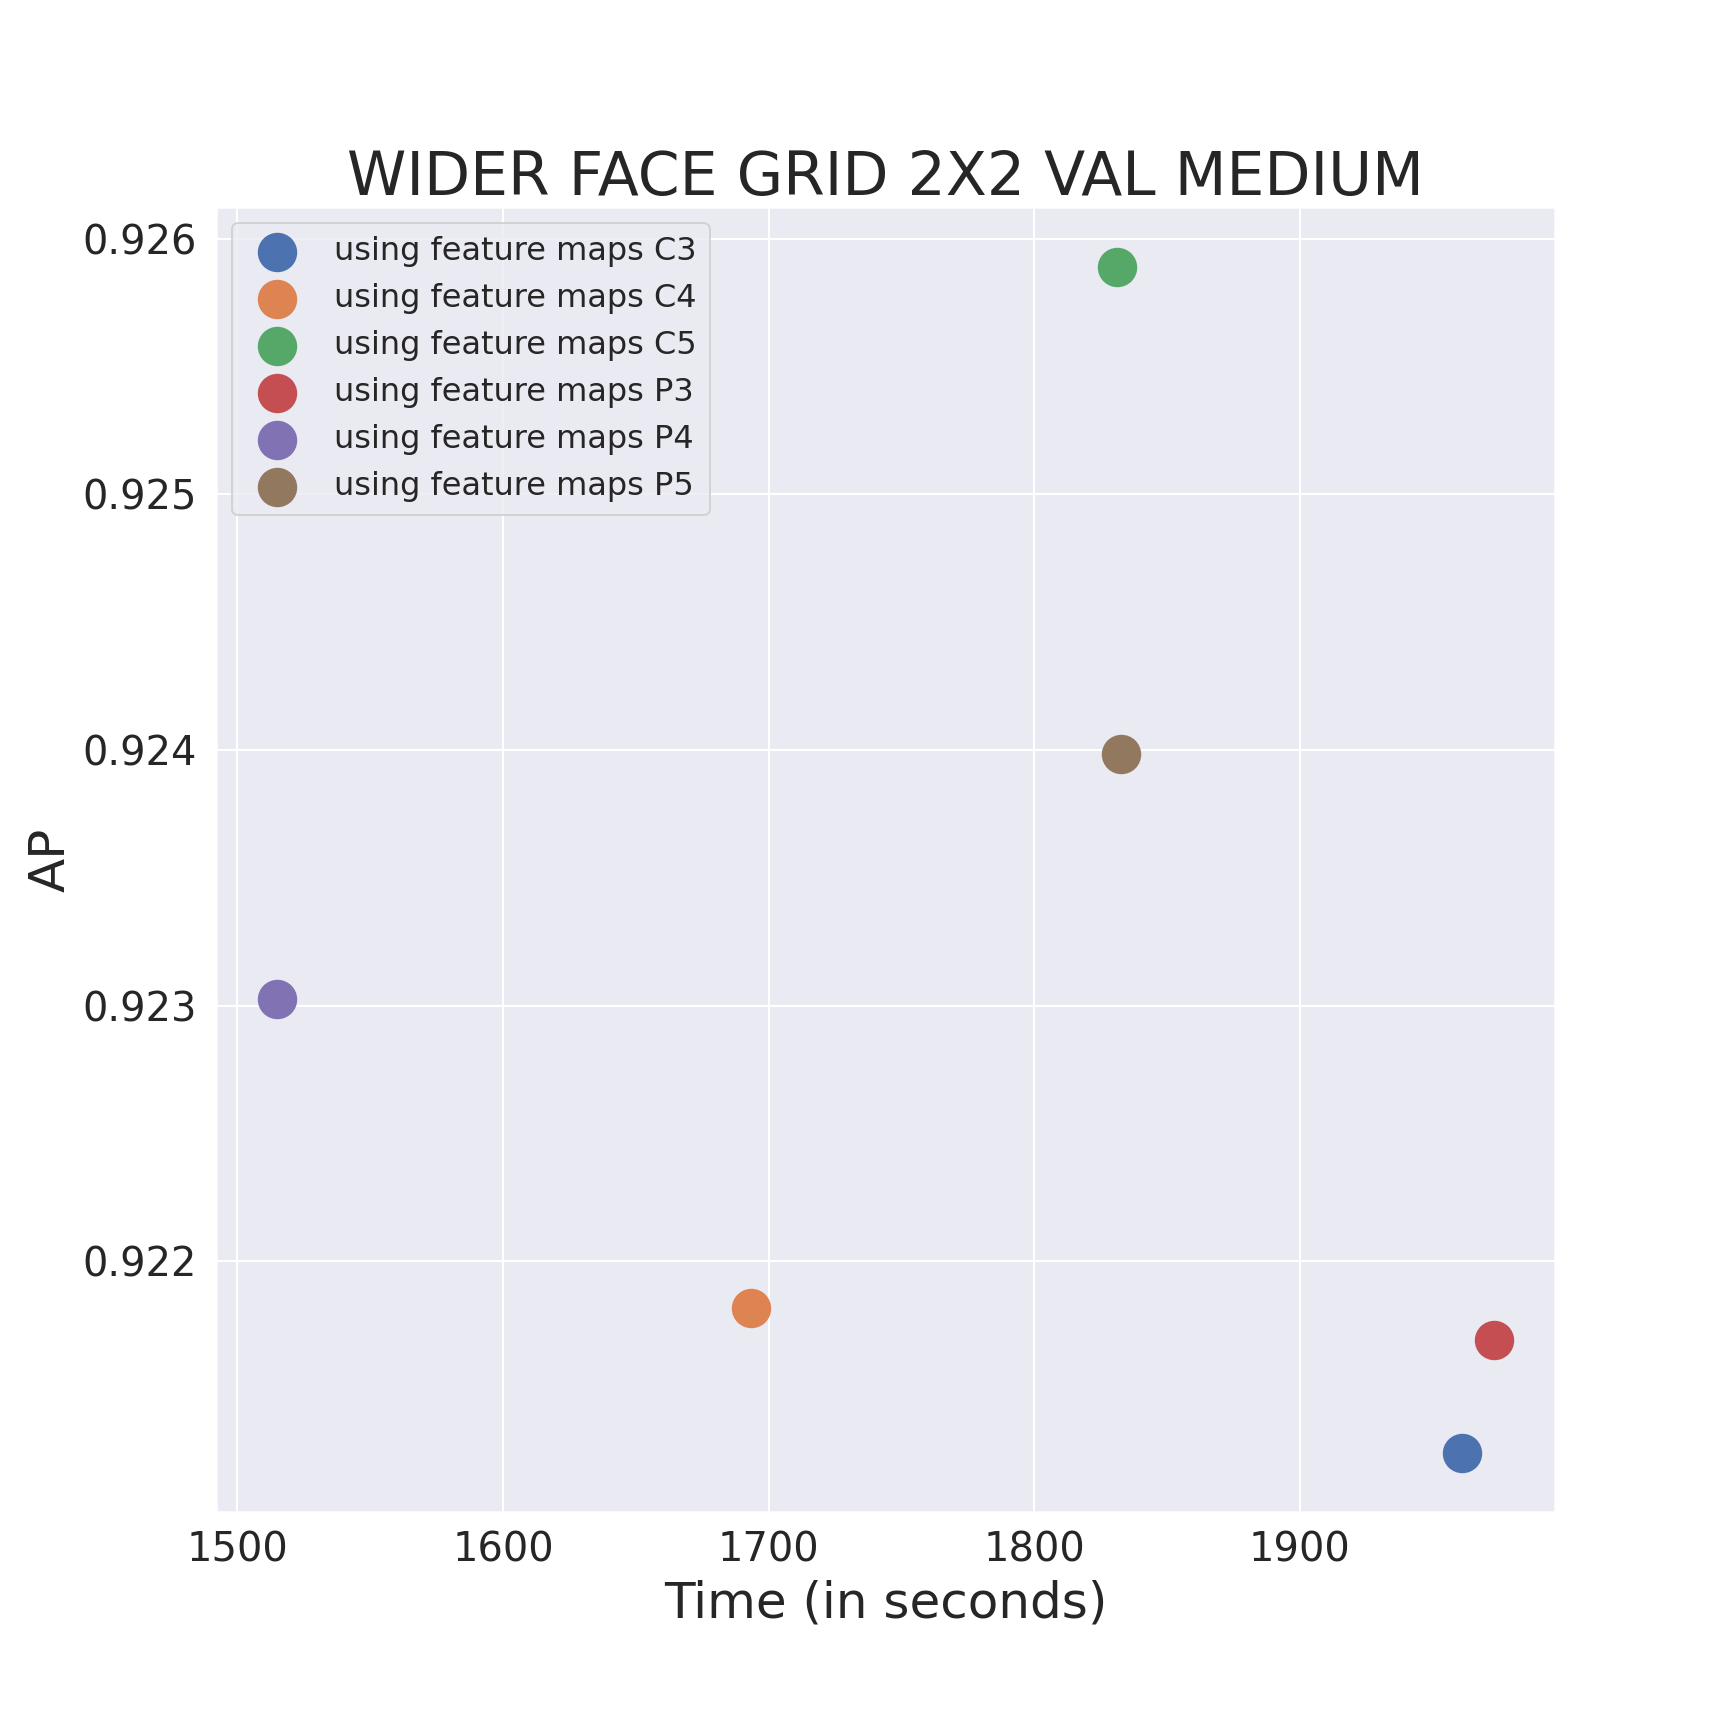
\includegraphics[width=7.3cm]{images/retinafocus_widerface_2k_val_medium_fpn}} 
        \subfigure[]{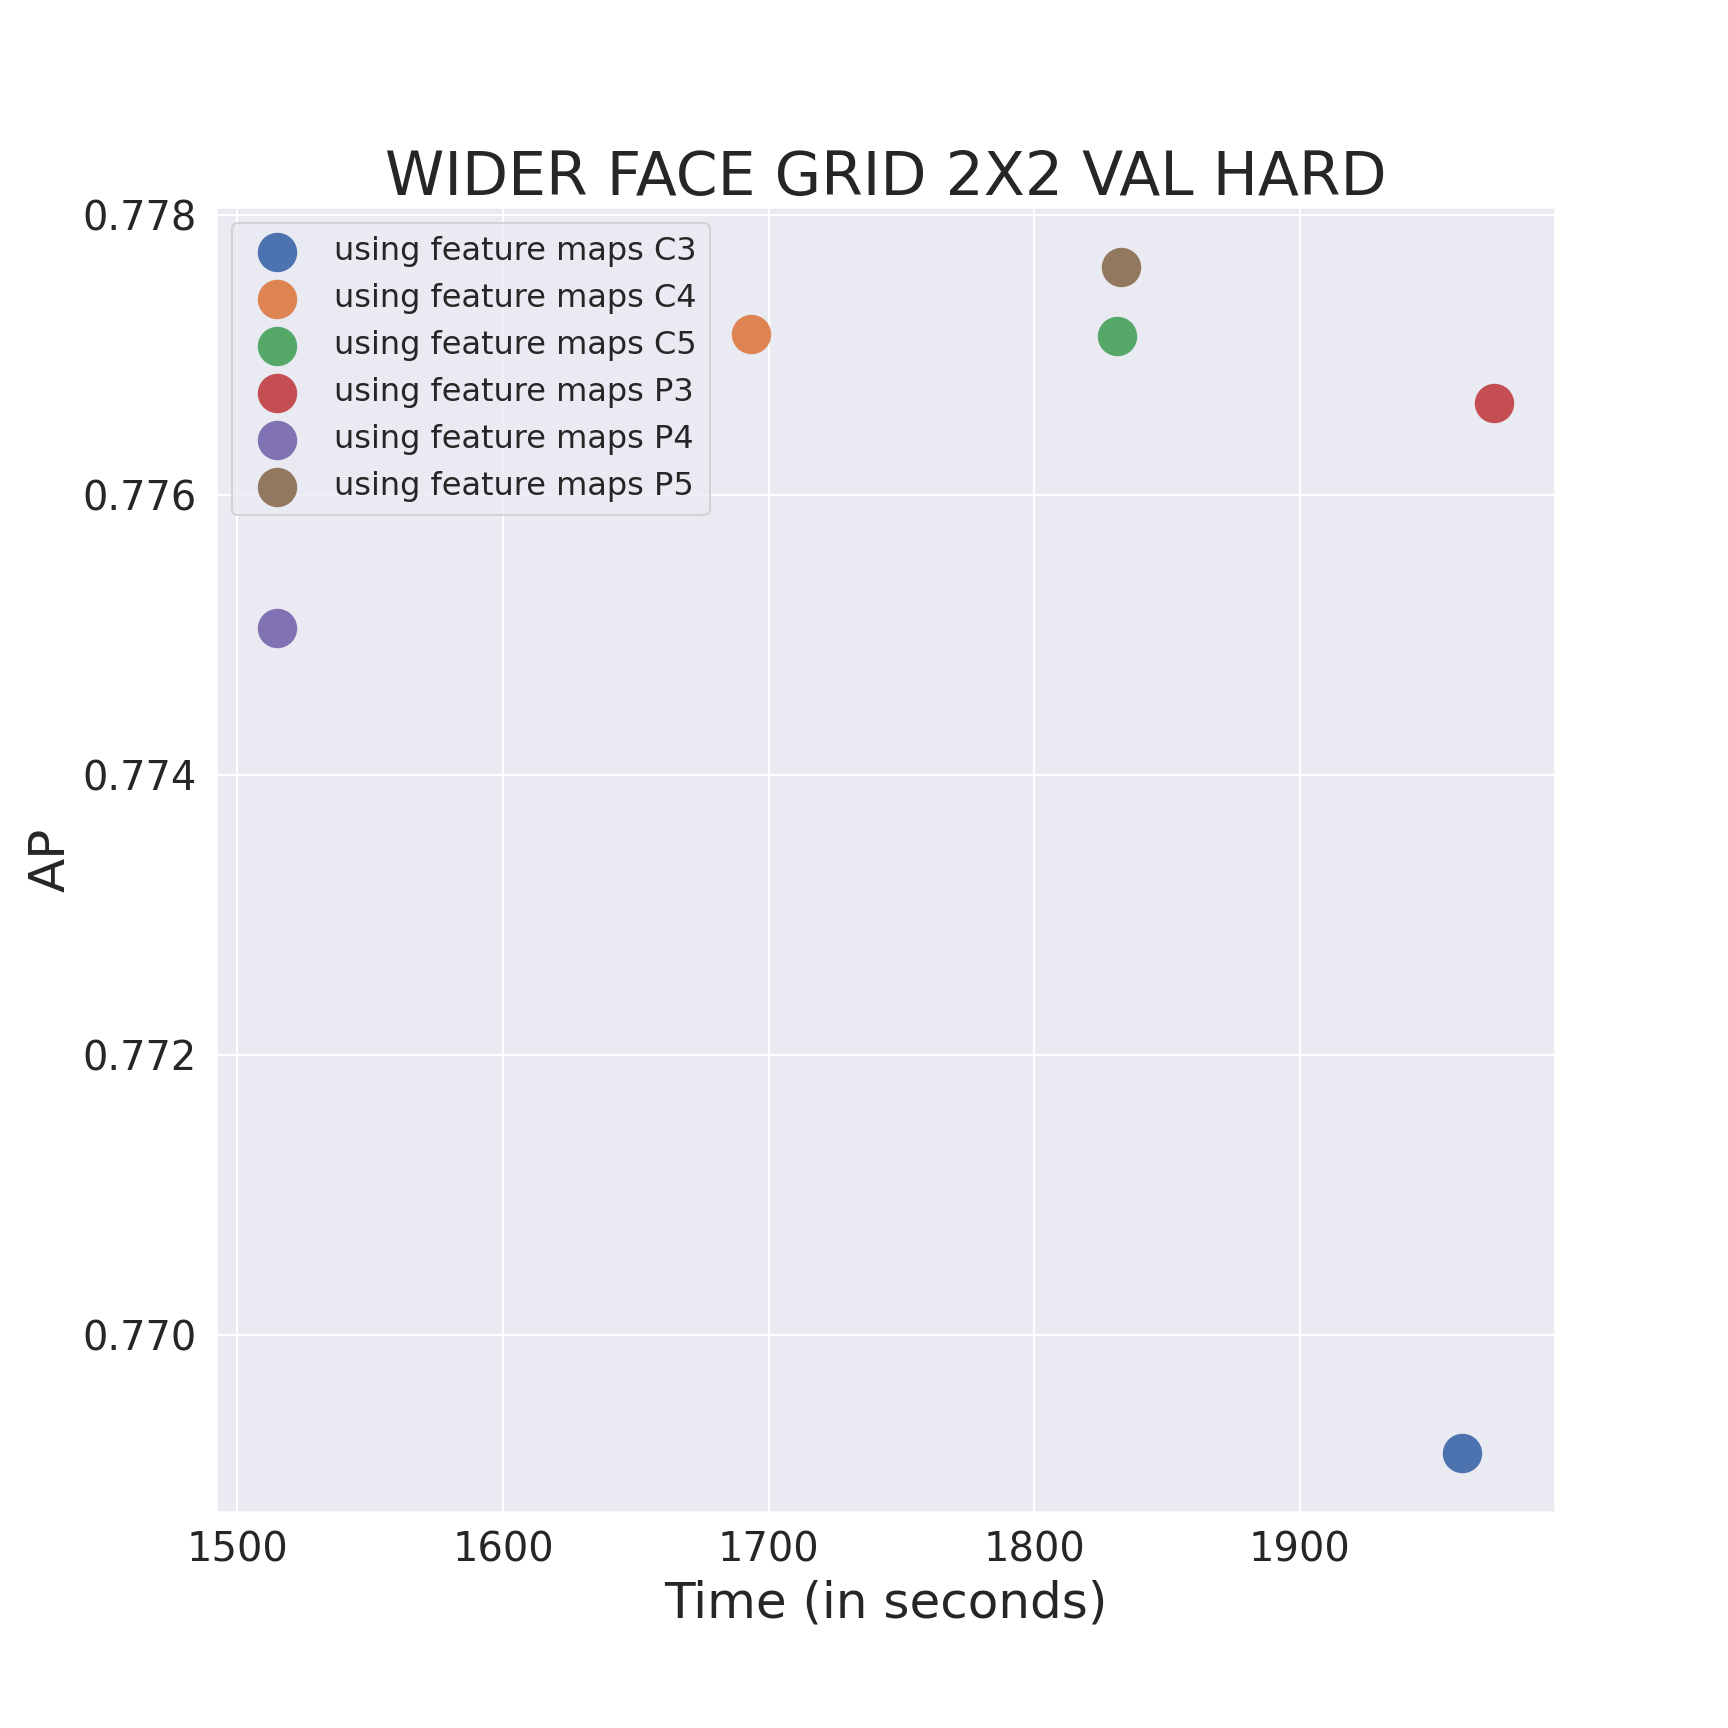
\includegraphics[width=7.3cm]{images/retinafocus_widerface_2k_val_hard_fpn}} 
        \caption{Kết quả so sánh các cấu hình sử dụng các bản đồ đặc trưng\index{bản đồ đặc trưng} của FPN làm đầu vào cho nhánh tập trung đối tượng\index{nhánh tập trung đối tượng} trên ba bộ dữ liệu WIDER FACE kích thước lớn lưới $2 X 2$ val easy (a), medium (b) và hard (c)}
        \label{fig:retinafocus_widerface_2k_val_fpn}
    \end{figure}

    \noindent
    Đối với bộ WIDER FACE kích thước lớn lưới $2 X 2$, ta có cấu hình tuỳ chỉnh gồm hai vòng lặp dự đoán với kích thước ảnh tương ứng của mỗi vòng lặp lần lượt là [800, 1200] điểm ảnh\index{điểm ảnh} và [1600, 2400] điểm ảnh\index{điểm ảnh}. \\
    Hai cấu hình đạt độ chính xác cao nhất vẫn là cấu hình sử dụng bản đồ đặc trưng\index{bản đồ đặc trưng} ${P}_{5}$ và cấu hình sử dụng bản đồ đặc trưng\index{bản đồ đặc trưng} ${C}_{5}$ với thời gian thực hiện toàn bộ quá trình dự đoán trên cả bộ dữ liệu lần lượt là 1832 và 1831 giây.
    Đối với bộ dữ liệu này, trong khi cấu hình sử dụng bản đồ đặc trưng\index{bản đồ đặc trưng} ${P}_{5}$ cho kết quả tốt hơn trên bộ WIDER FACE kích thước lớn lưới $2 X 2$ val easy và hard thì cấu hình sử dụng bản đồ đặc trưng\index{bản đồ đặc trưng} ${C}_{5}$ cho kết quả tốt hơn trên bộ WIDER FACE kích thước lớn lưới $2 X 2$ val medium.
    Tuy nhiên, đối với bộ WIDER FACE kích thước lớn lưới $2 X 2$ val hard, kết quả của cấu hình sử dụng bản đồ đặc trưng\index{bản đồ đặc trưng} ${C}_{4}$ và ${P}_{3}$ cho kết quả khá tiệm cận với cấu hình sử dụng bản đồ đặc trưng\index{bản đồ đặc trưng} ${C}_{5}$.

    \begin{figure}[H]
        \centering
        \subfigure[]{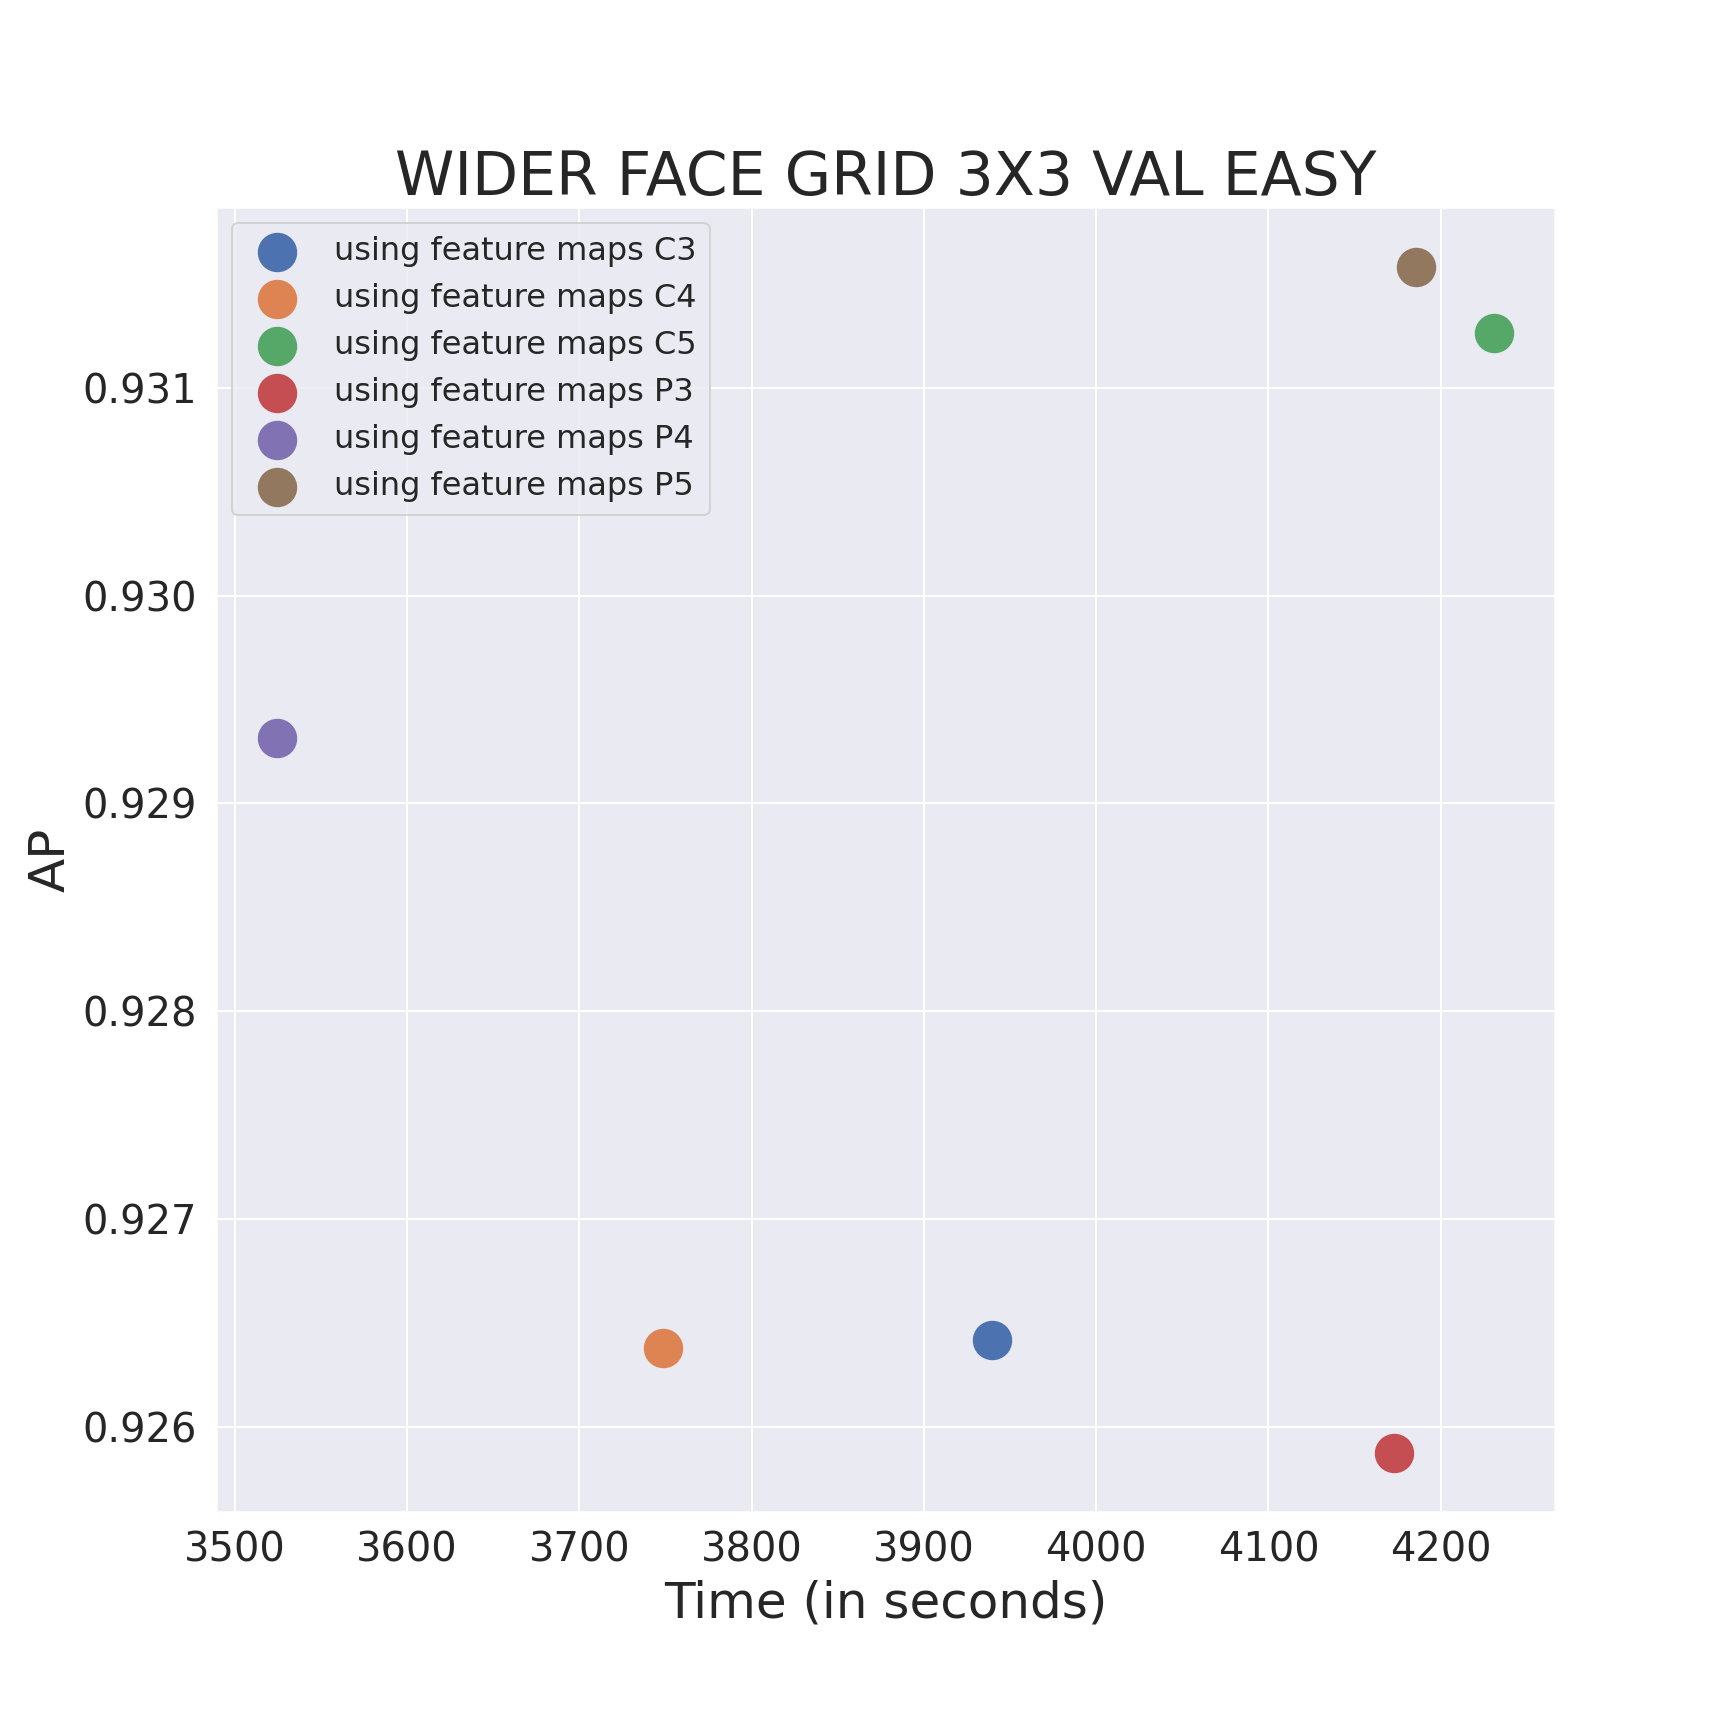
\includegraphics[width=7.3cm]{images/retinafocus_widerface_3k_val_easy_fpn}} 
        \subfigure[]{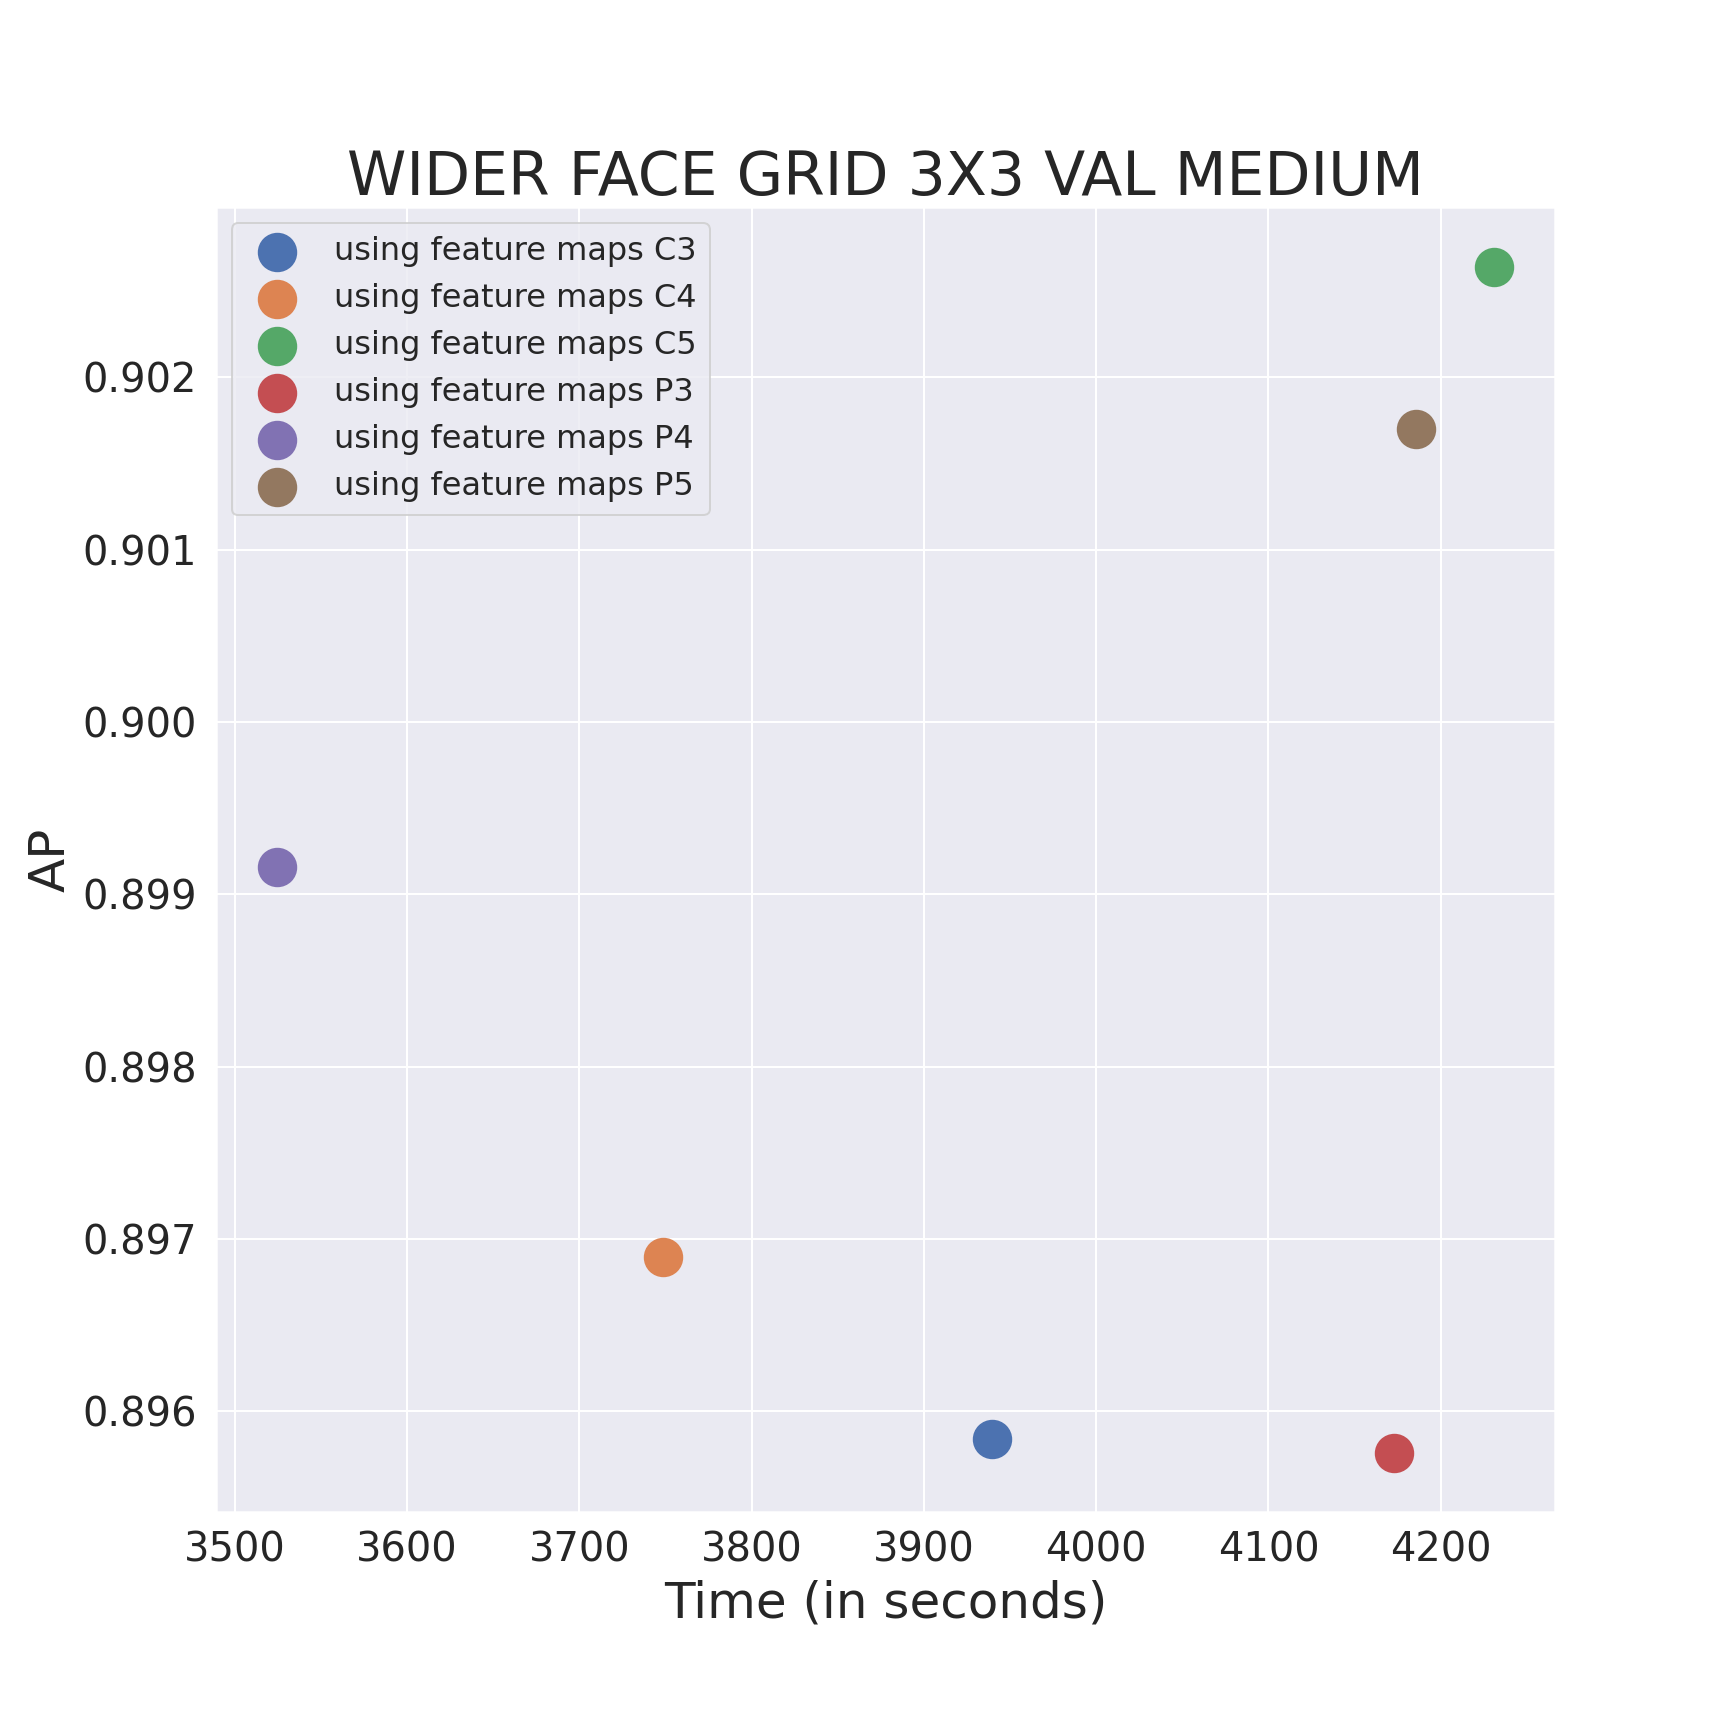
\includegraphics[width=7.3cm]{images/retinafocus_widerface_3k_val_medium_fpn}} 
        \subfigure[]{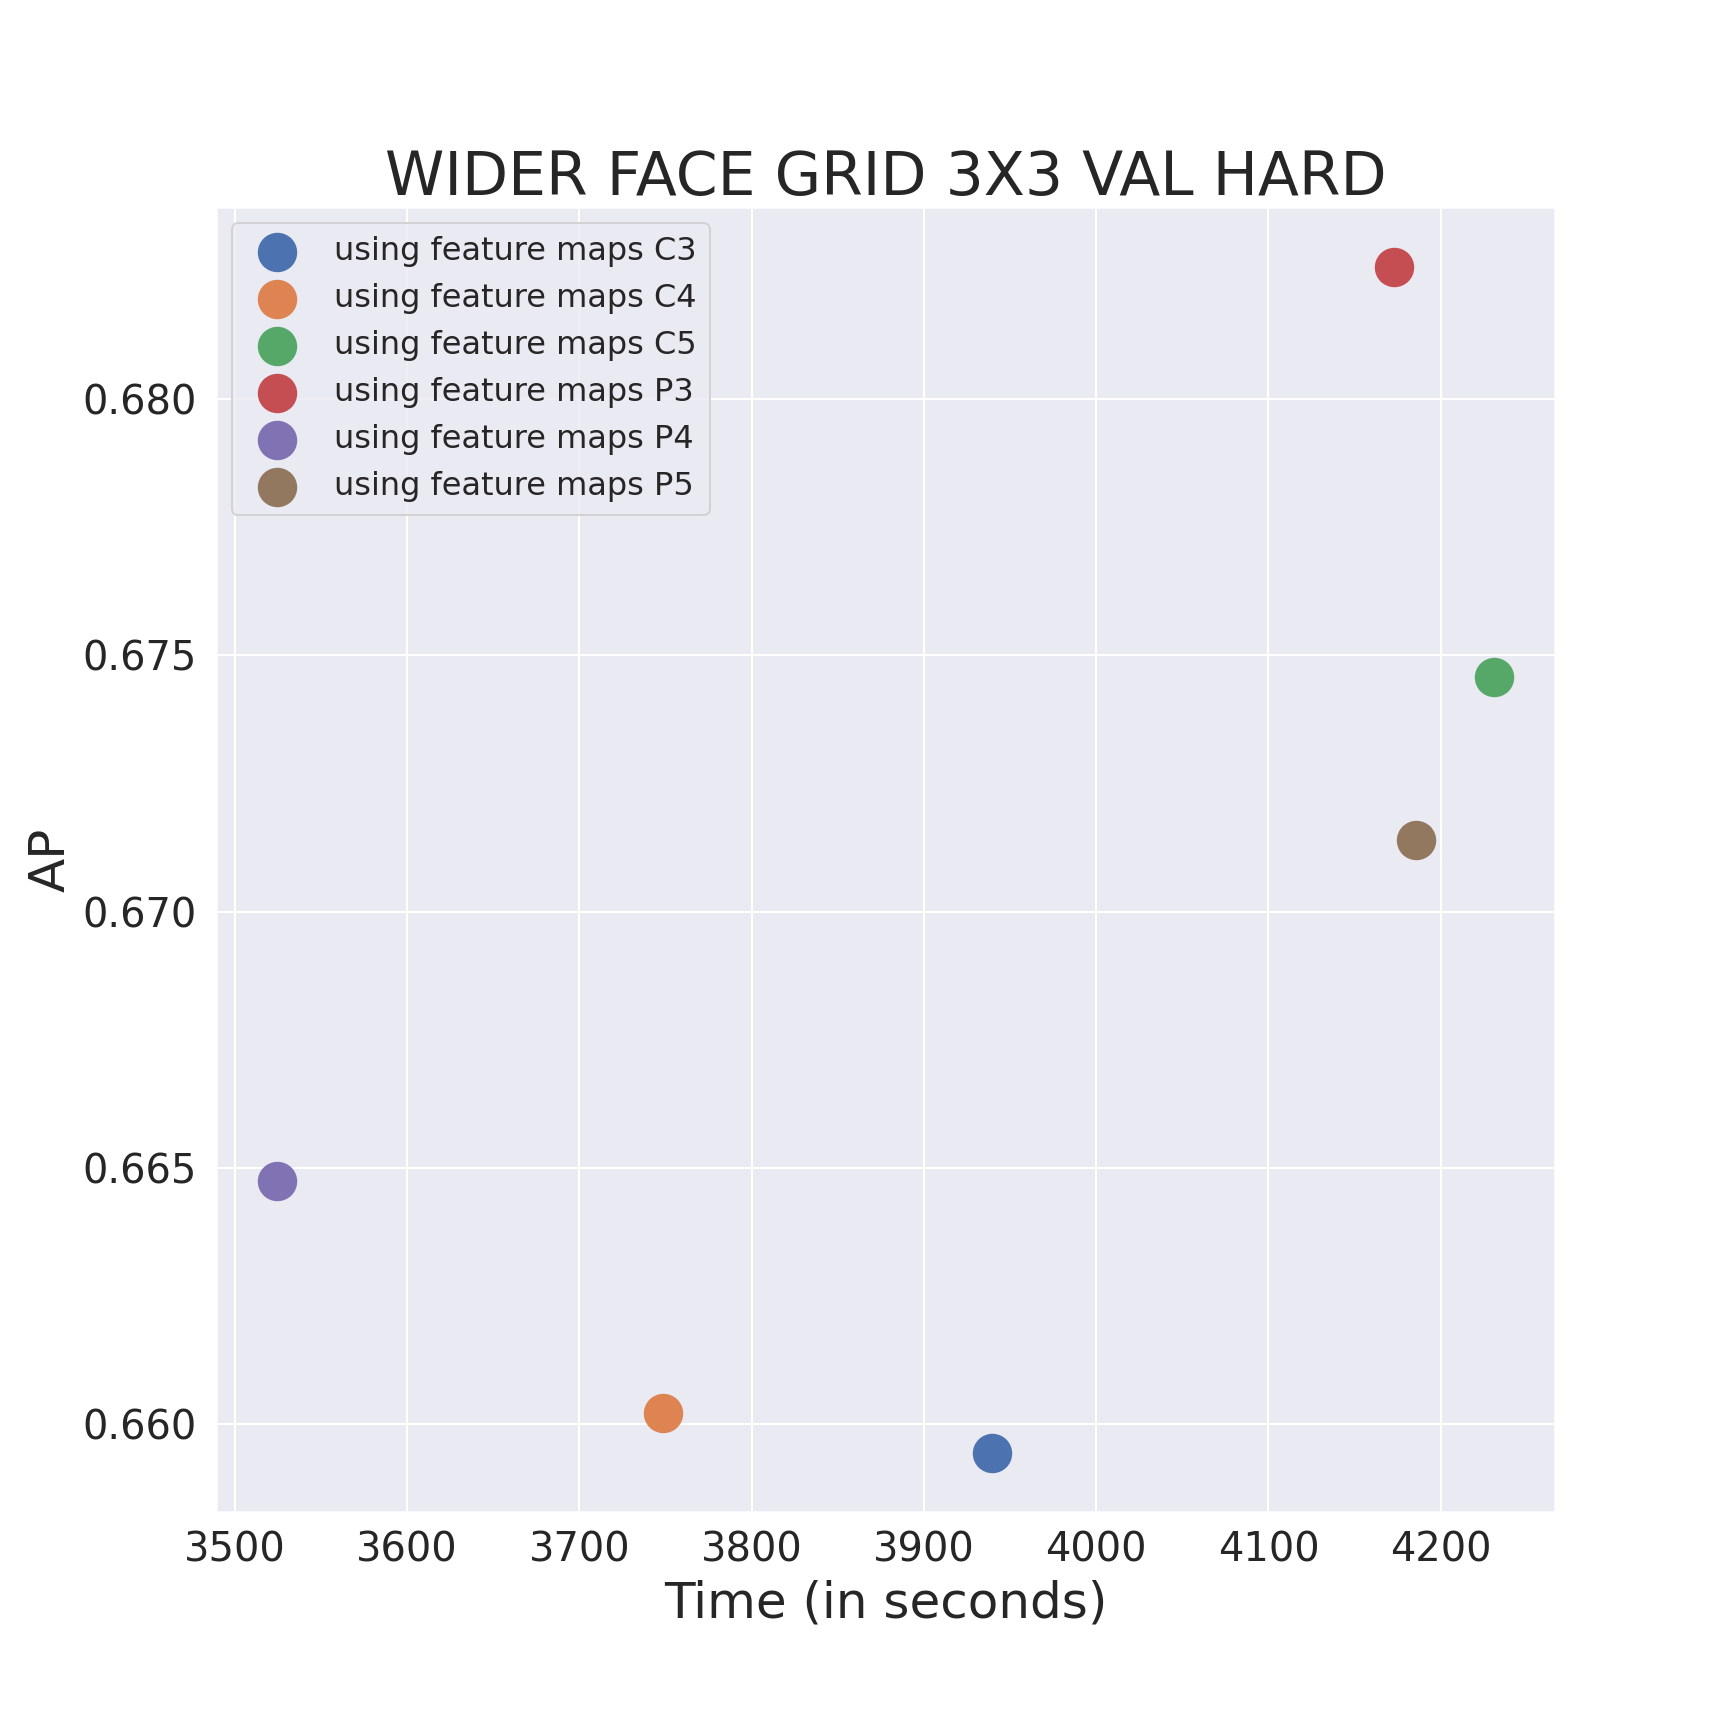
\includegraphics[width=7.3cm]{images/retinafocus_widerface_3k_val_hard_fpn}} 
        \caption{Kết quả so sánh các cấu hình sử dụng các bản đồ đặc trưng\index{bản đồ đặc trưng} của FPN làm đầu vào cho nhánh tập trung đối tượng\index{nhánh tập trung đối tượng} trên ba bộ dữ liệu WIDER FACE kích thước lớn lưới $3 X 3$ val easy (a), medium (b) và hard (c)}
        \label{fig:retinafocus_widerface_3k_val_fpn}
    \end{figure}

    \noindent
    Đối với bộ WIDER FACE kích thước lớn lưới $3 X 3$, ta có cấu hình tuỳ chỉnh gồm hai vòng lặp dự đoán với kích thước ảnh tương ứng của mỗi vòng lặp lần lượt là [800, 1200] điểm ảnh\index{điểm ảnh} và [1600, 2400] điểm ảnh\index{điểm ảnh}. \\
    Từ đó, các cấu hình đạt độ chính xác cao nhất đã có những sự thay đổi.
    Đối với bộ WIDER FACE kích thước lớn lưới $3 X 3$ easy, cấu hình sử dụng bản đồ đặc trưng\index{bản đồ đặc trưng} ${P}_{5}$ cho kết quả tốt nhất với thời gian thực hiện toàn bộ quá trình dự đoán trên cả bộ dữ liệu lần lượt là 4185 giây.
    Đối với bộ WIDER FACE kích thước lớn lưới $3 X 3$ medium, cấu hình sử dụng bản đồ đặc trưng\index{bản đồ đặc trưng} ${C}_{5}$ cho kết quả tốt nhất với thời gian thực hiện toàn bộ quá trình dự đoán trên cả bộ dữ liệu lần lượt là 4231 giây.
    Đối với bộ WIDER FACE kích thước lớn lưới $3 X 3$ hard, cấu hình sử dụng bản đồ đặc trưng\index{bản đồ đặc trưng} ${P}_{3}$ cho kết quả tốt nhất, vượt qua khá xa hai cấu hình sử dụng bản đồ đặc trưng\index{bản đồ đặc trưng} ${P}_{5}$ và ${C}_{5}$, với thời gian thực hiện toàn bộ quá trình dự đoán trên cả bộ dữ liệu lần lượt là 4172 giây.

    \noindent
    Kết luận đối với thí nghiệm này, đối với mỗi bộ dữ liệu khác nhau như WIDER FACE thông thường, WIDER FACE kích thước lớn lưới $2 X 2$ hay $3 X 3$ và các bộ dữ liệu con easy, medium và hard, kết quả về cấu hình đạt độ chính xác cao nhất khác nhau, phụ thuộc vào kích thước ảnh đầu vào và tỷ lệ giữa kích thước của hộp giới hạn\index{hộp giới hạn} và kích thước của ảnh đầu vào tương ứng.

    \subsubsection*{Thí nghiệm so sánh cấu hình tốt nhất của mô hình RetinaFocus với các cấu hình của mô hình RetinaFace}
    Mô hình RetinaFocus mất khoảng 48 tiếng dành cho quá trình huấn luyện khi sử dụng thư viện Pytorch với phần cứng là một GPU NVIDIA GeForce RTX 2080 Ti. \\
    Đối với mô hình RetinaFace, trong khuôn khổ của luận văn, tôi không thực hiện tại quá trình huấn luyện của mô hình mà chỉ sử dụng kết quả mô hình đã có sẵn của tác giả.
    
    \noindent
    Các cấu hình của mô hình RetinaFace sử dụng trong thí nghiệm này bao gồm: \\
    - Cấu hình sử dụng chiến lược Image Pyramids kết hợp với việc lật ảnh đầu vào trong quá trình dự đoán, ký hiệu là \textit{RetinaFace with Image Pyramids and Flip}. \\
    - Cấu hình không sử dụng chiến lược Image Pyramids mà chỉ sử dụng một tuỳ chỉnh kích thước ảnh duy nhất là [1600, 2150], ký hiệu là \textit{RetinaFace with single scale [1600, 2150]}.

    \noindent
    Cấu hình của mô hình RetinaFocus sử dụng trong thí nghiệm này là cấu hình cho kết quả tốt nhất trên từng bộ dữ liệu.
    Cụ thể, đối với bộ dữ liệu WIDER FACE val easy và medium, ta chọn cấu hình sử dụng bản đồ đặc trưng\index{bản đồ đặc trưng} $P_5$ được ký hiệu là \textit{RetinaFocus using feature maps P5}. \\
    Đối với bộ dữ liệu WIDER FACE val hard, ta chọn cấu hình sử dụng bản đồ đặc trưng\index{bản đồ đặc trưng} $C_5$ được ký hiệu là \textit{RetinaFocus using feature maps C5}. \\
    Cả hai cấu hình trên đều thực hiện vòng lặp dự đoán năm lần, với các kích thước của ảnh đầu vào của mô hình tương đương với kích thước ảnh gốc ban đầu lần lượt với mỗi vòng lặp là [500, 750] điểm ảnh\index{điểm ảnh}, [800, 1200] điểm ảnh\index{điểm ảnh}, [1100, 1650] điểm ảnh\index{điểm ảnh}, [1400, 2100] điểm ảnh\index{điểm ảnh}, [1700, 2550] điểm ảnh\index{điểm ảnh}.

    \noindent
    Trong so sánh tại hình \ref{fig:retinafocus_widerface_val_rtnf}, các cấu hình của mô hình RetinaFocus cho kết quả về độ chính xác thấp hơn so với các cấu hình của mô hình RetinaFace khoảng từ 1\% - 2\%.
    Tuy nhiên, xét trên khía cạnh tốc độ, các cấu hình của mô hình RetinaFocus cho kết quả nhanh hơn khoảng hơn 8 lần so với cấu hình tốt nhất là \textit{RetinaFace with Image Pyramids and Flip} và nhanh hơn khoảng 1.5 lần so với cấu hình \textit{RetinaFace with single scale [1600, 2150]}.

    \begin{figure}[H]
        \centering
        \subfigure[]{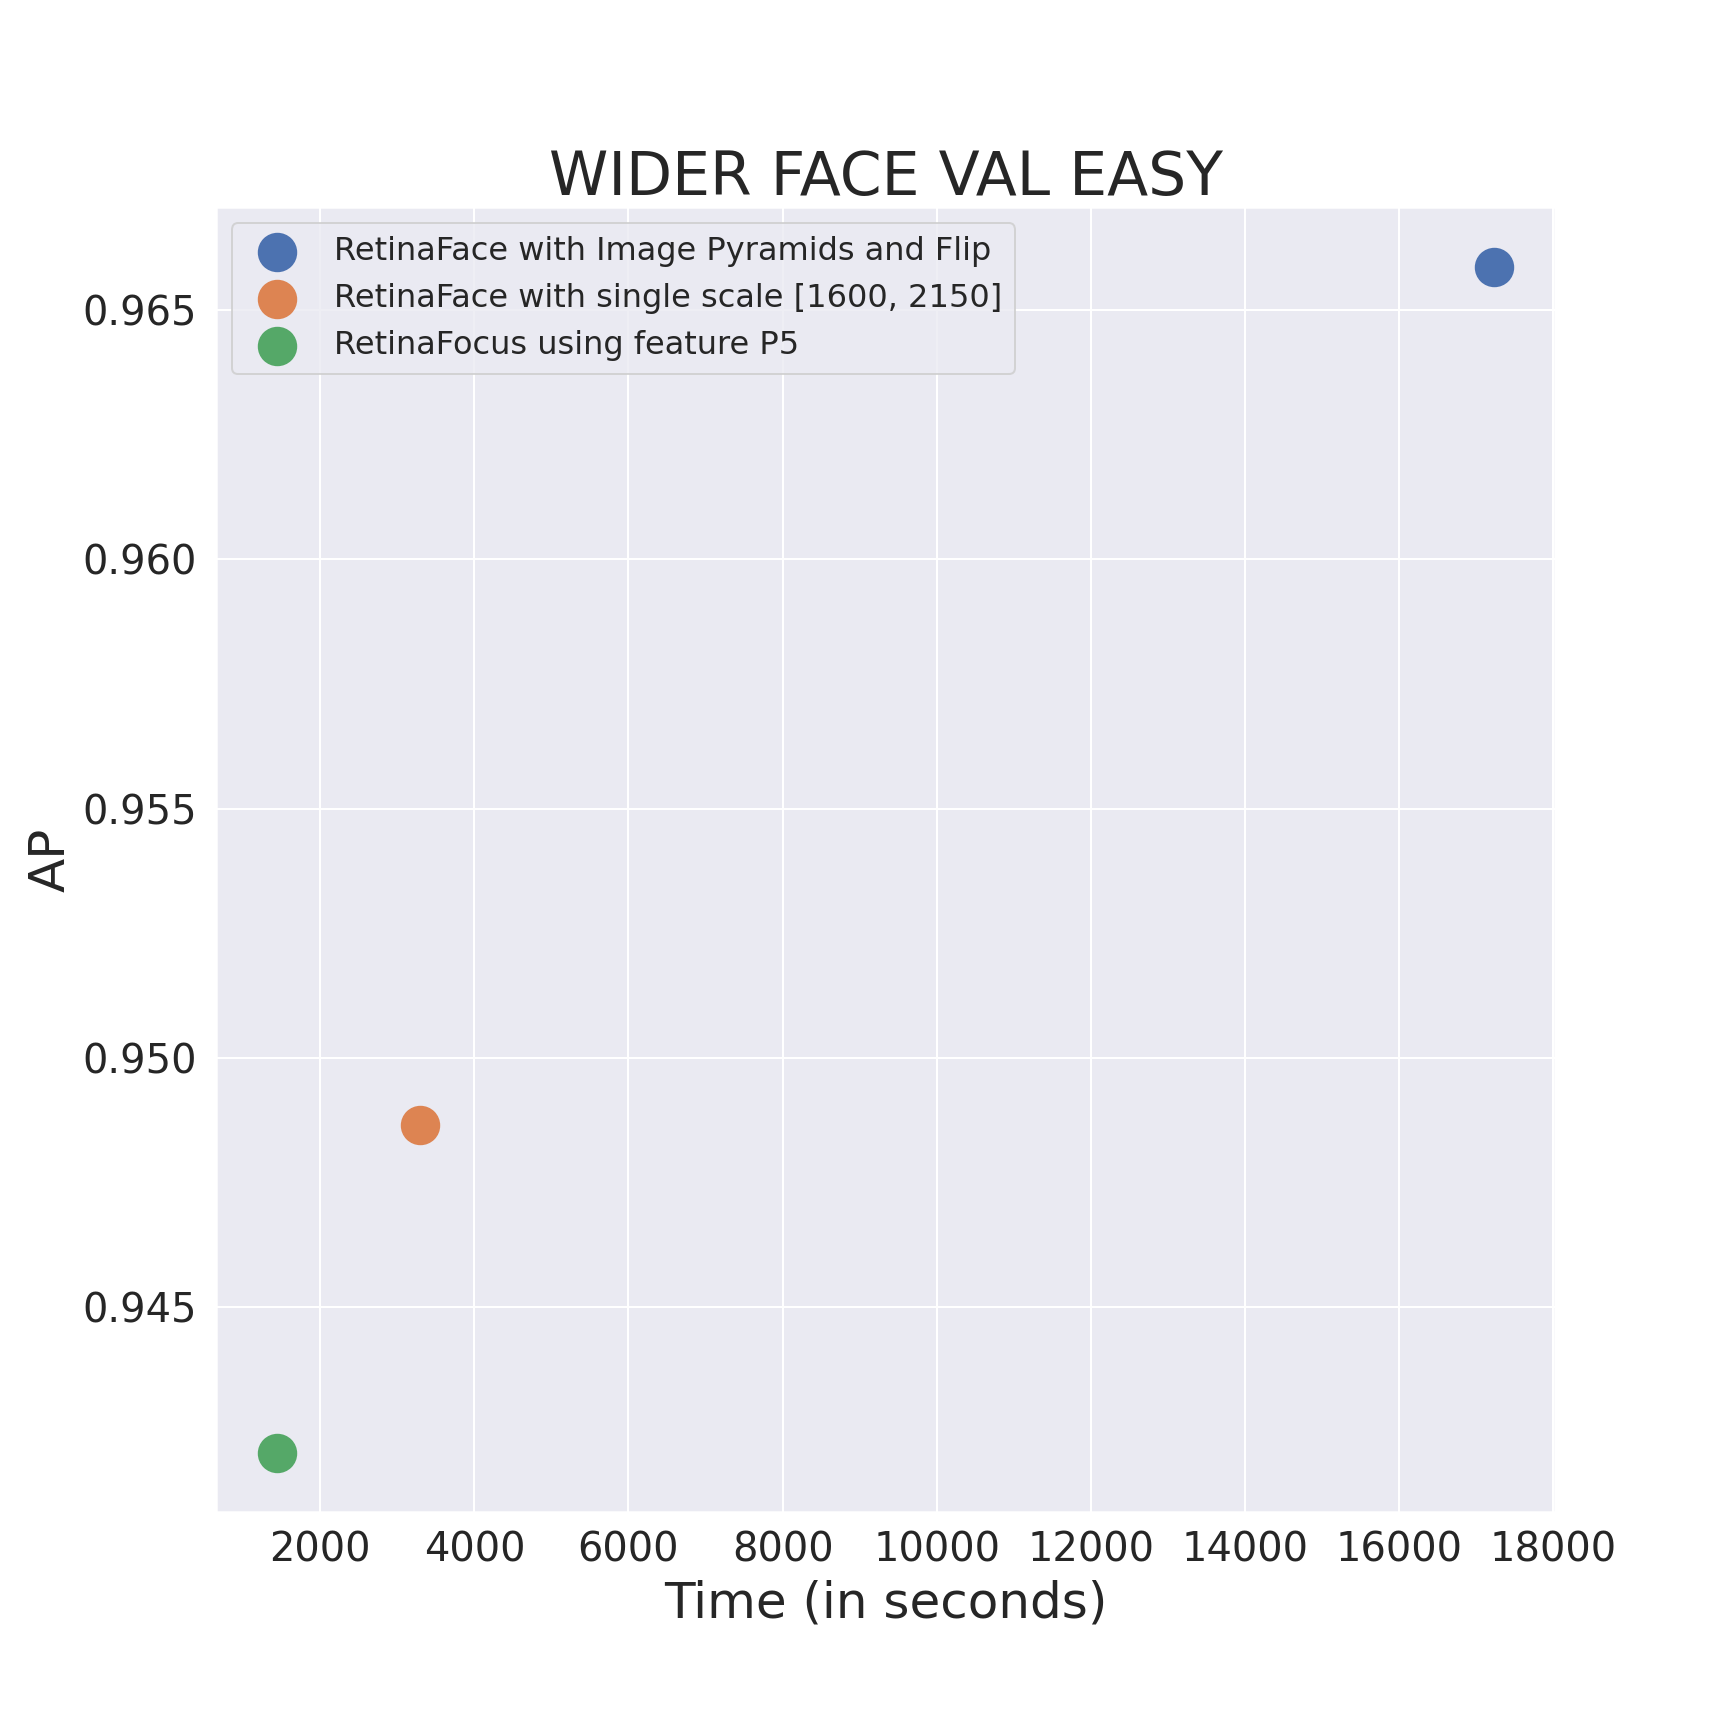
\includegraphics[width=7.3cm]{images/retinafocus_widerface_val_easy_rtnf}} 
        \subfigure[]{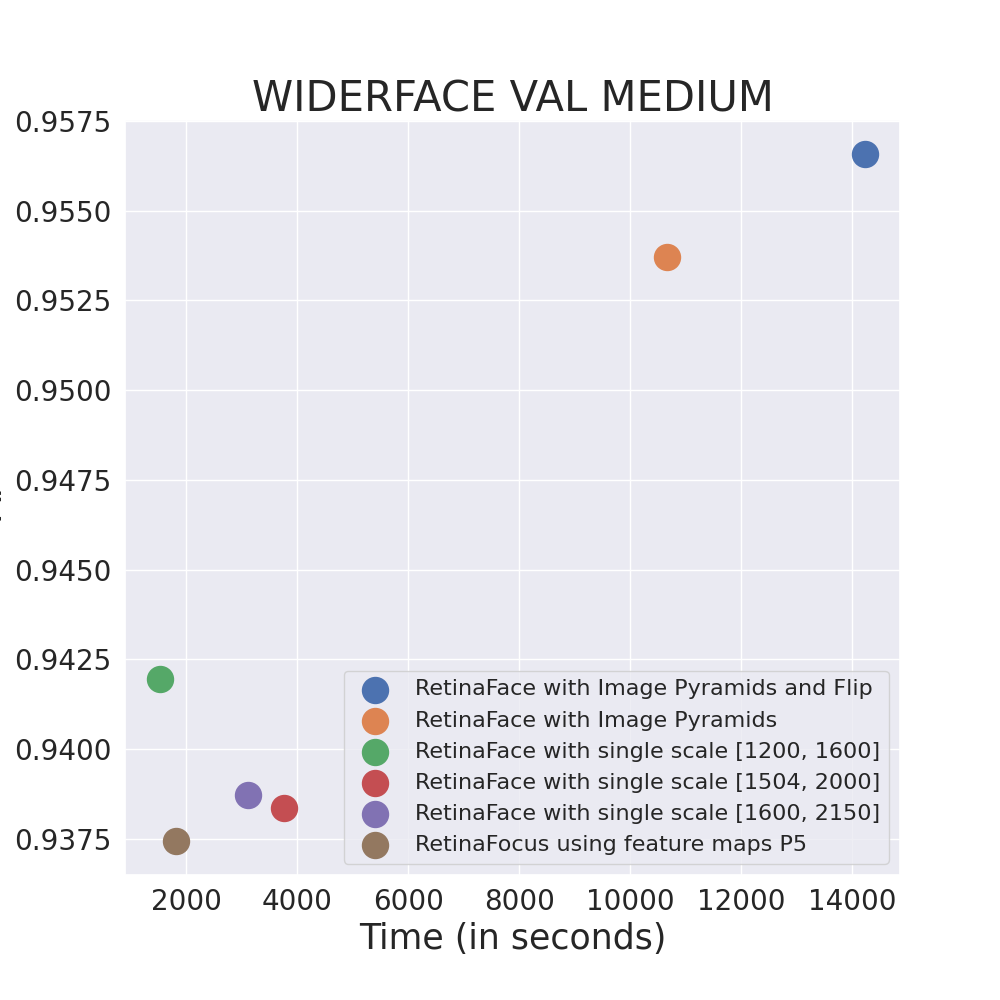
\includegraphics[width=7.3cm]{images/retinafocus_widerface_val_medium_rtnf}} 
        \subfigure[]{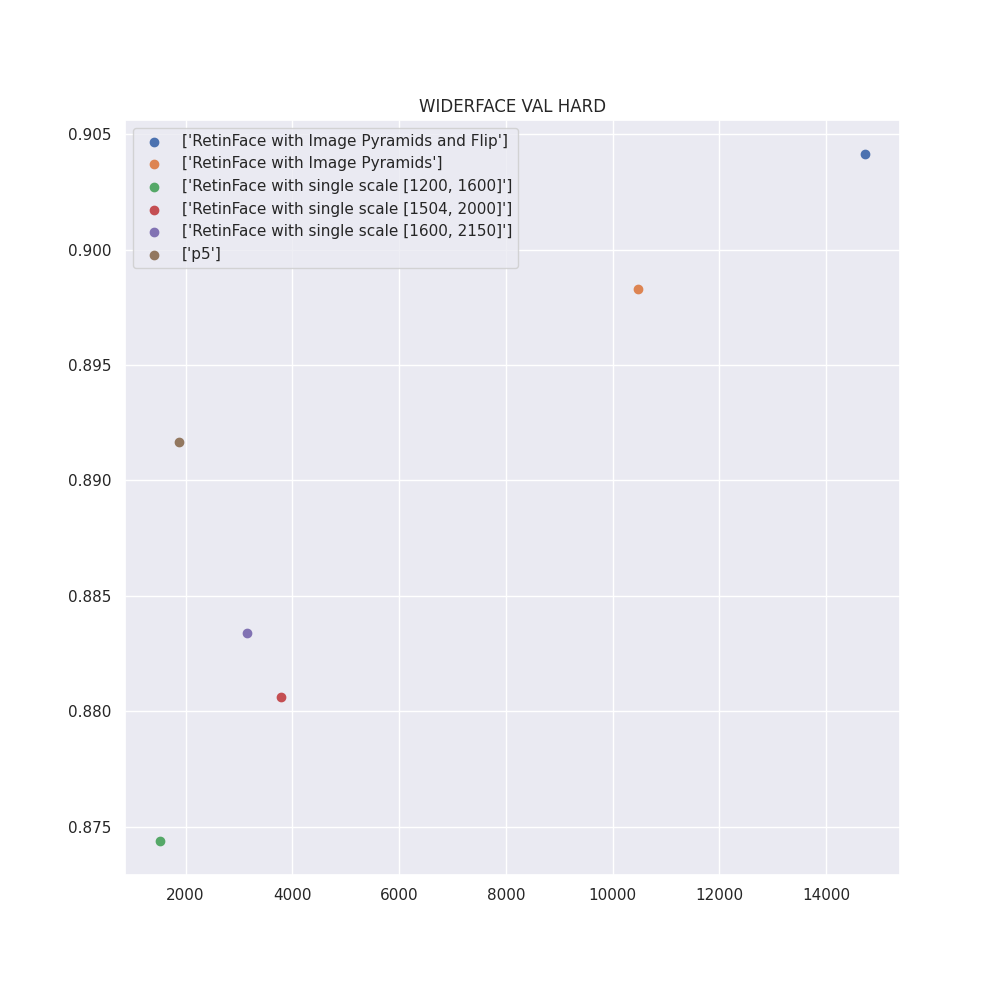
\includegraphics[width=7.3cm]{images/retinafocus_widerface_val_hard_rtnf}} 
        \caption{Kết quả so sánh cấu hình tốt nhất của RetinaFocus với các cấu hình của RetinaFace trên ba bộ dữ liệu WIDER FACE val easy (a), medium (b) và hard (c)}
        \label{fig:retinafocus_widerface_val_rtnf}
    \end{figure}

    \noindent
    Trên bộ dữ liệu WIDER FACE kích thước lớn lưới $2 X 2$, kết quả so sánh được thể hiện tại hình \ref{fig:retinafocus_widerface_2k_val_rtnf}, ta vẫn sử dụng hai cấu hình \textit{RetinaFace with Image Pyramids and Flip} và \textit{RetinaFace with single scale [1600, 2150]} đại diện cho mô hình RetinaFace.

    \noindent
    Đối với mô hình RetinaFocus, ta sử dụng cấu hình tốt nhất tương ứng với từng bộ dữ liệu.
    Ta chọn cấu hình sử dụng bản đồ đặc trưng\index{bản đồ đặc trưng} $P_5$ được ký hiệu là \textit{RetinaFocus using feature maps P5} dành cho bộ WIDER FACE kích thước lớn lưới $2 X 2$ val easy và hard. \\
    Ta chọn cấu hình sử dụng bản đồ đặc trưng\index{bản đồ đặc trưng} $C_5$ được ký hiệu là \textit{RetinaFocus using feature maps C5} dành cho bộ WIDER FACE kích thước lớn lưới $2 X 2$ val medium. \\
    Cả hai cấu hình trên đều thực hiện vòng lặp dự đoán hai lần, với các kích thước của ảnh đầu vào của mô hình tương đương với kích thước ảnh gốc ban đầu lần lượt với mỗi vòng lặp là [800, 1200] điểm ảnh\index{điểm ảnh} và [1600, 2400] điểm ảnh\index{điểm ảnh}.

    \noindent
    Trong thí nghiệm này, các kết quả của các cấu hình của mô hình RetinaFocus cũng cho kết quả về độ chính xác thấp hơn so với các cấu hình của mô hình RetinaFace khoảng từ 1\% - 2\%.
    Trên khía cạnh tốc độ, các cấu hình của mô hình RetinaFocus cho kết quả nhanh hơn khoảng hơn 6 lần so với cấu hình tốt nhất là \textit{RetinaFace with Image Pyramids and Flip} và nhanh hơn khoảng 1.2 lần so với cấu hình \textit{RetinaFace with single scale [1600, 2150]}. \\
    Điều này thể hiện rằng các tham số trong chiến lược dự đoán của các cấu hình của mô hình RetinaFocus được lựa chọn chưa thật sự chính xác và phù hợp với mô hình, dẫn đến kết quả dự đoán kém.

    \begin{figure}[H]
        \centering
        \subfigure[]{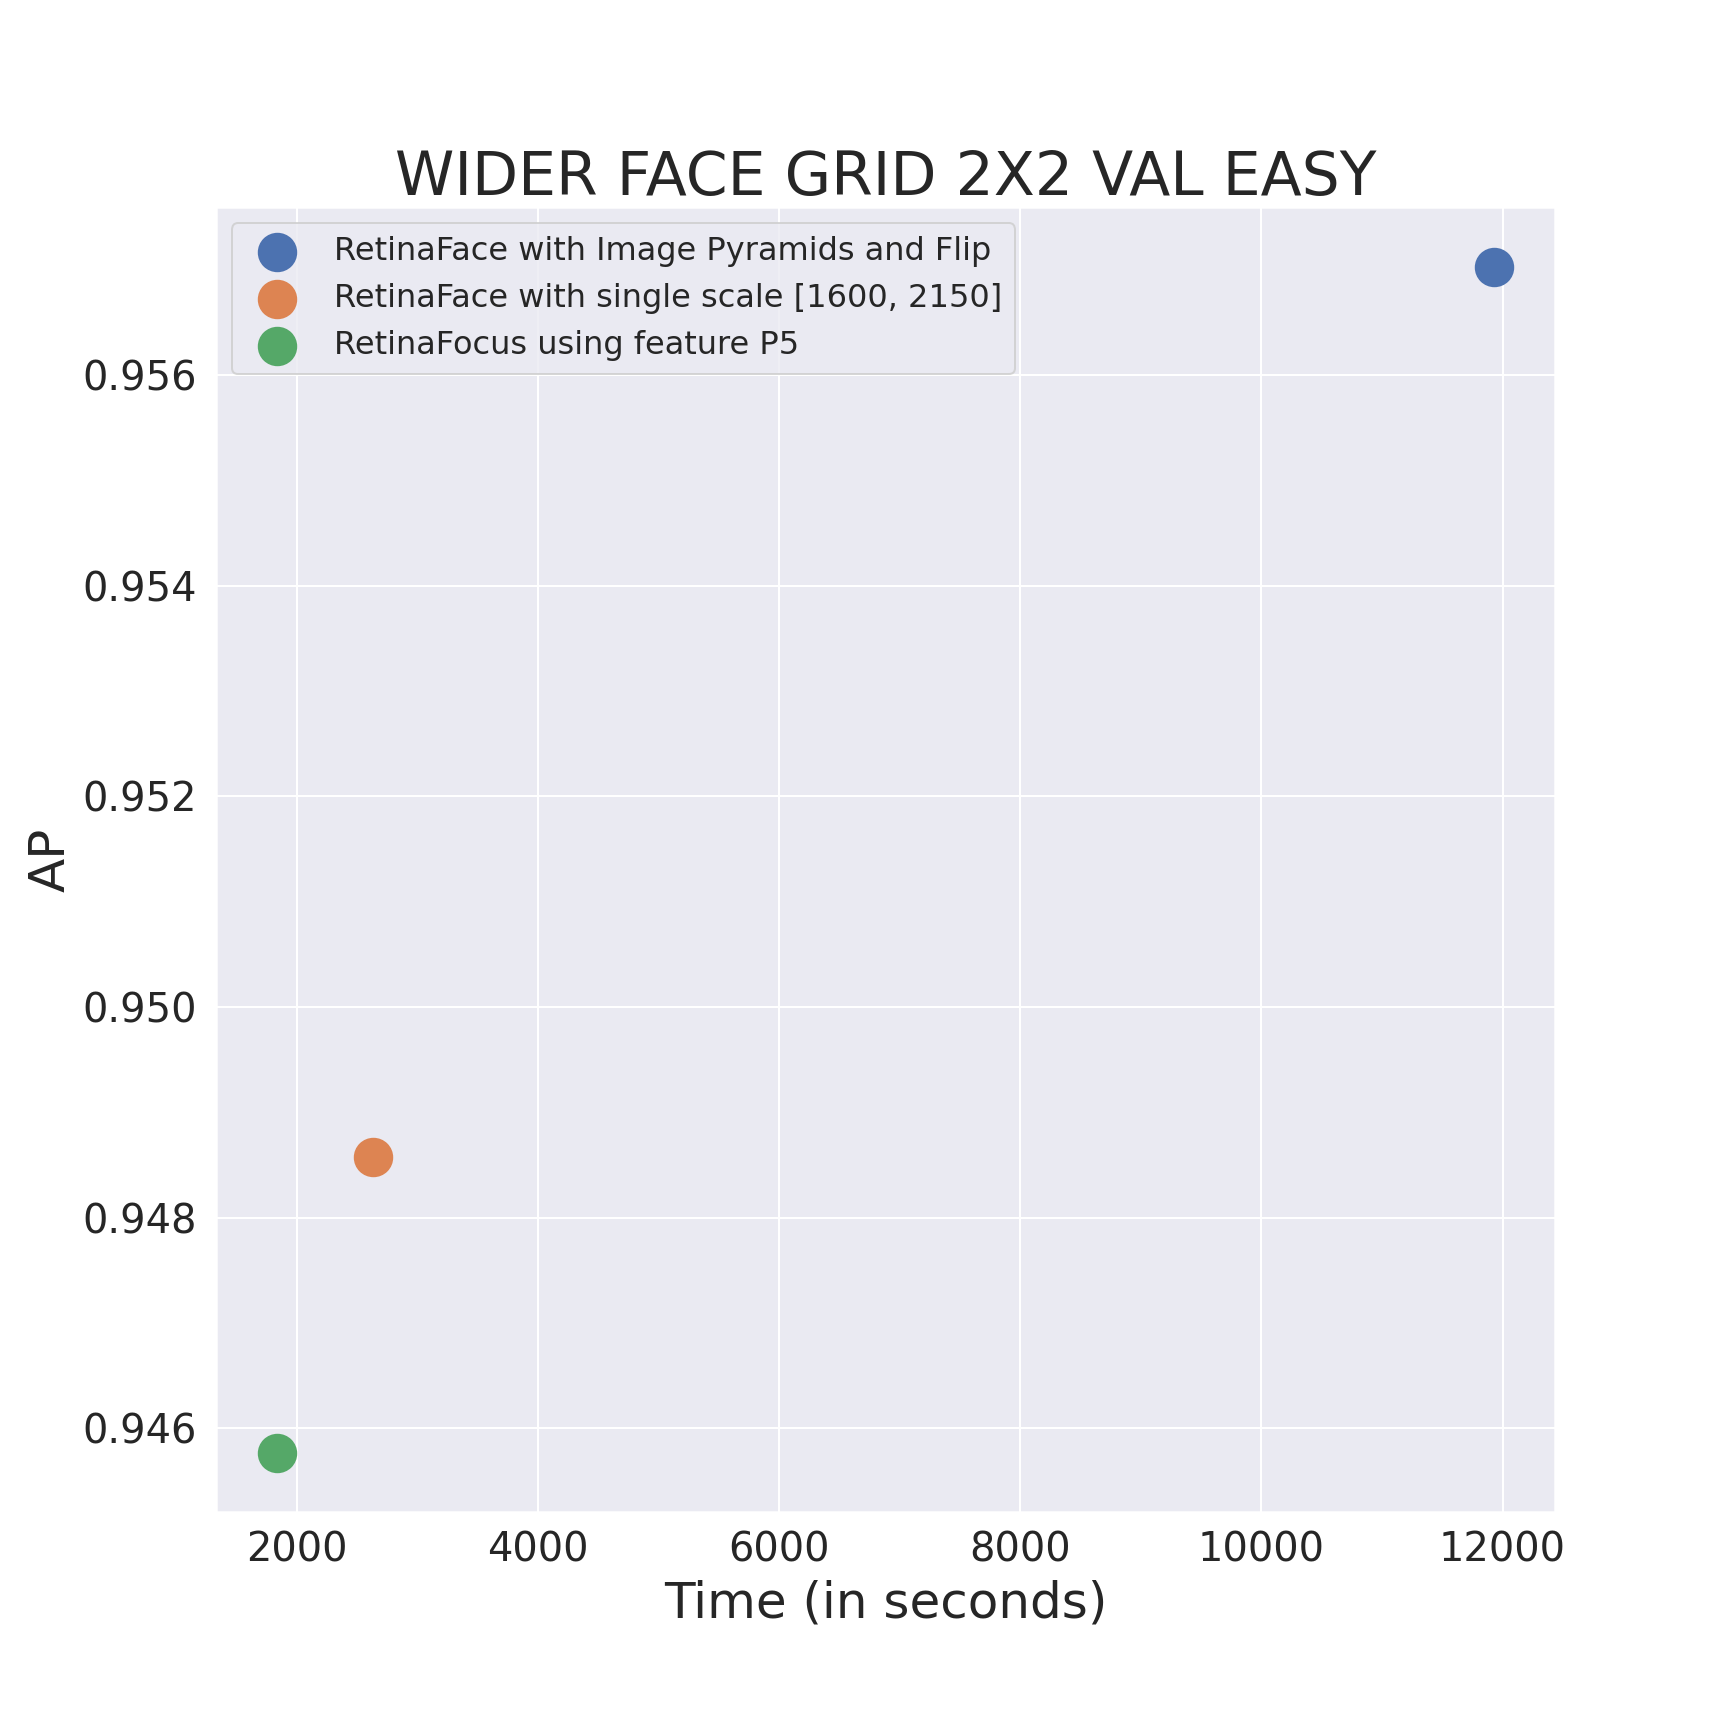
\includegraphics[width=7.3cm]{images/retinafocus_widerface_2k_val_easy_rtnf}} 
        \subfigure[]{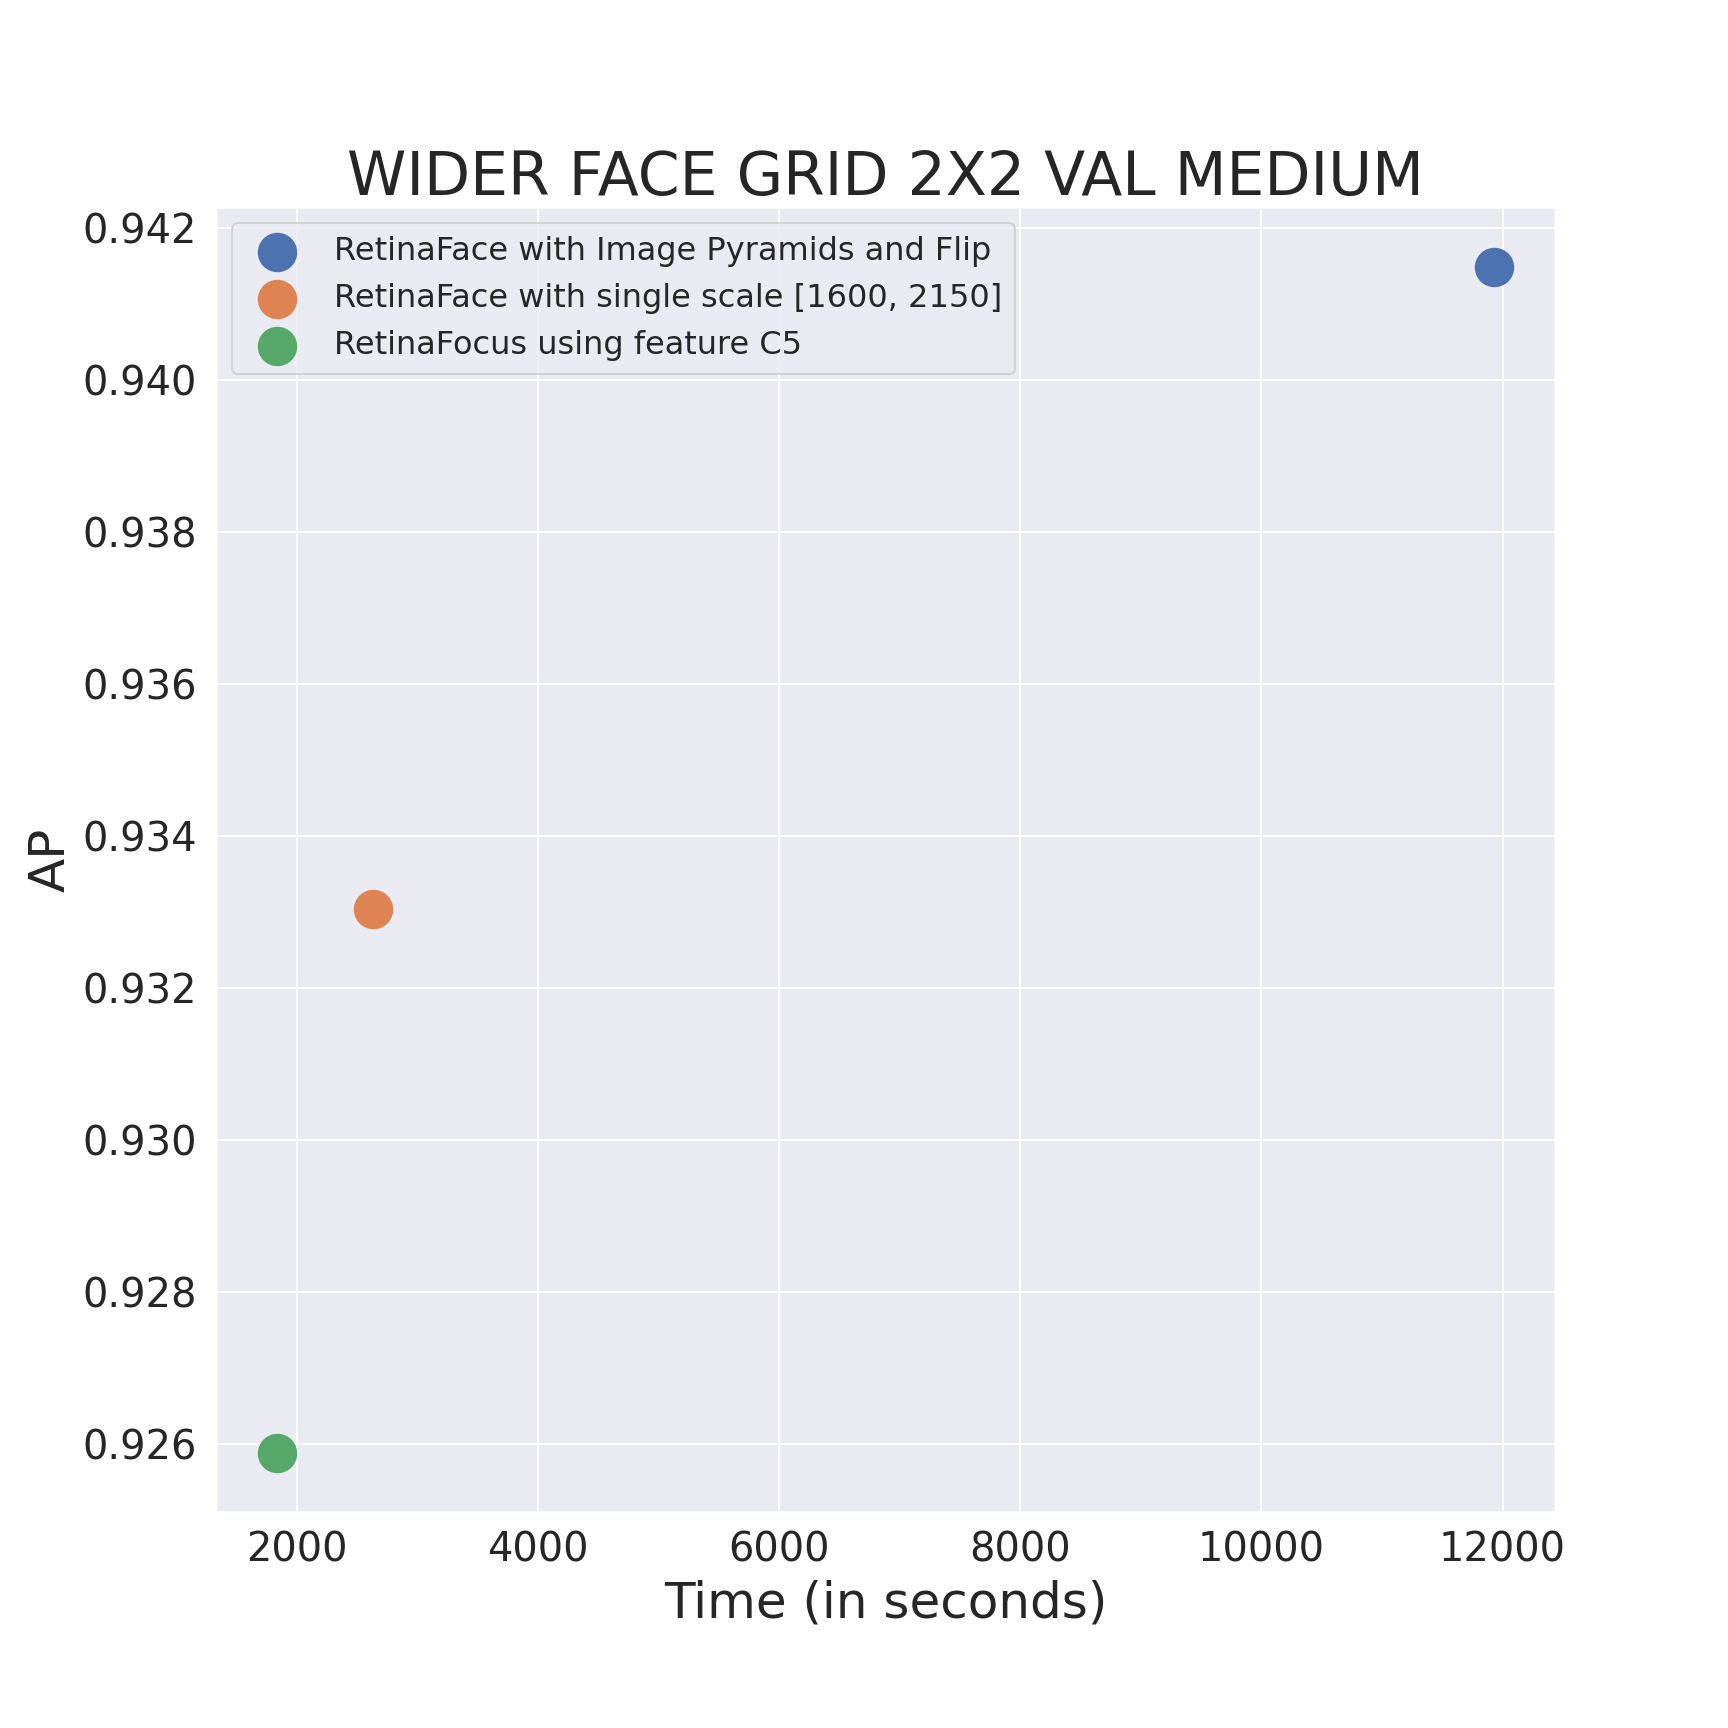
\includegraphics[width=7.3cm]{images/retinafocus_widerface_2k_val_medium_rtnf}} 
        \subfigure[]{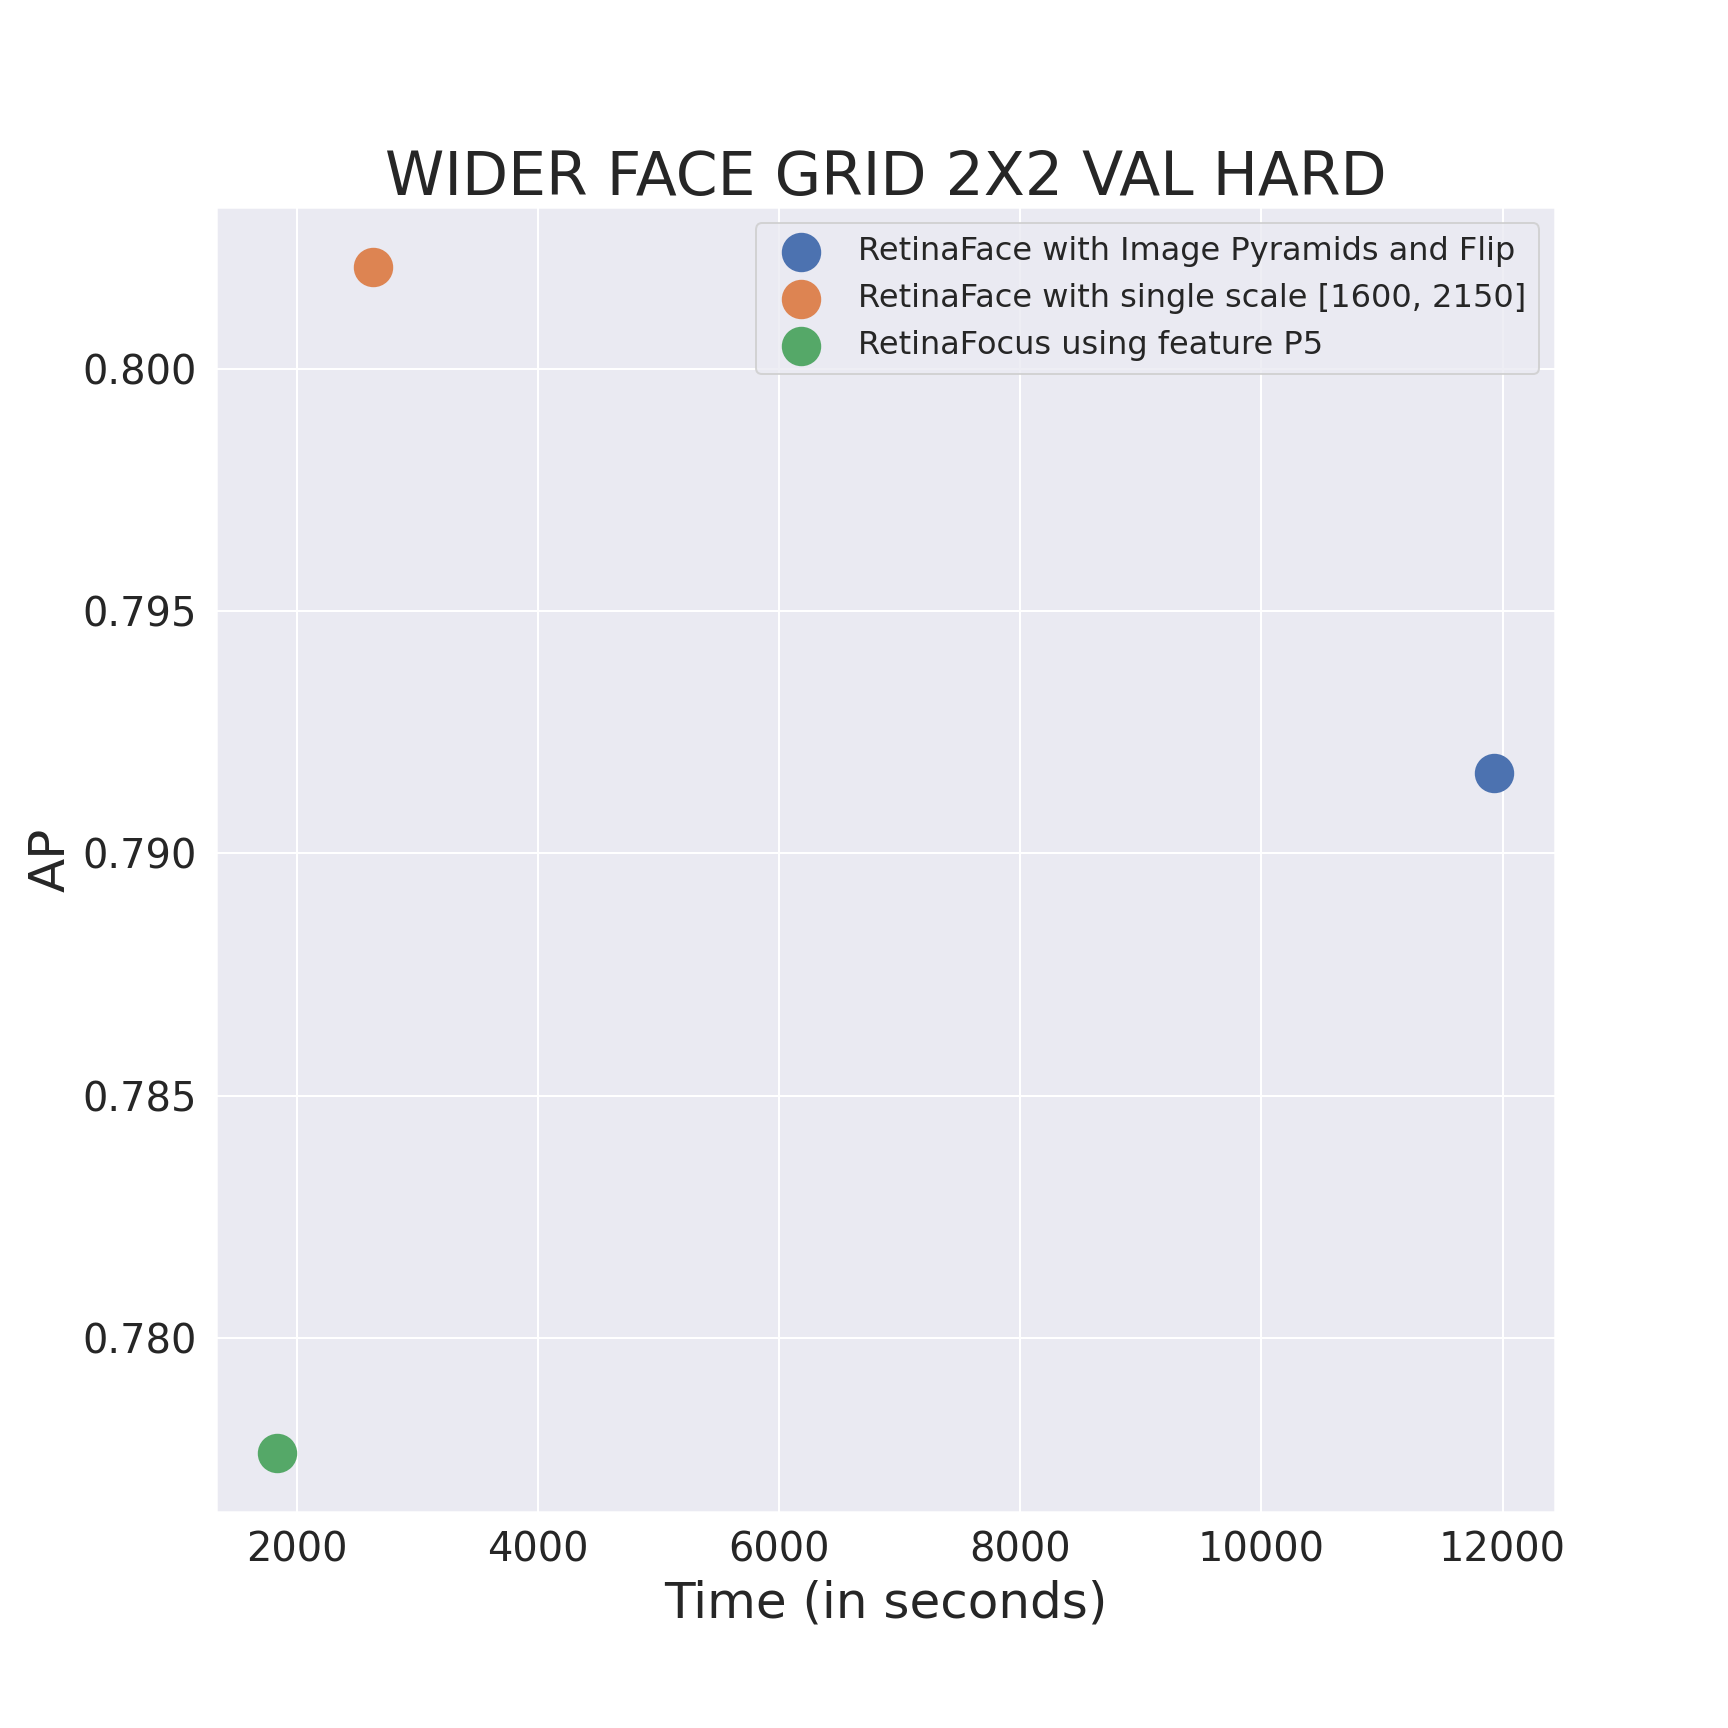
\includegraphics[width=7.3cm]{images/retinafocus_widerface_2k_val_hard_rtnf}} 
        \caption{Kết quả so sánh cấu hình tốt nhất của RetinaFocus với các cấu hình của RetinaFace trên ba bộ dữ liệu WIDER FACE kích thước lớn lưới $2 X 2$ val easy (a), medium (b) và hard (c)}
        \label{fig:retinafocus_widerface_2k_val_rtnf}
    \end{figure}

    \noindent
    Trên bộ dữ liệu WIDER FACE kích thước lớn lưới $3 X 3$, kết quả so sánh được thể hiện tại hình \ref{fig:retinafocus_widerface_3k_val_rtnf}, ta vẫn sử dụng hai cấu hình \textit{RetinaFace with Image Pyramids and Flip} và \textit{RetinaFace with single scale [1600, 2150]} đại diện cho mô hình RetinaFace.

    \noindent
    Đối với mô hình RetinaFocus, ta sử dụng cấu hình tốt nhất tương ứng với từng bộ dữ liệu. \\
    Ta chọn cấu hình sử dụng bản đồ đặc trưng\index{bản đồ đặc trưng} $P_5$ được ký hiệu là \textit{RetinaFocus using feature maps P5} dành cho bộ WIDER FACE kích thước lớn lưới $3 X 3$ val easy. \\
    Ta chọn cấu hình sử dụng bản đồ đặc trưng\index{bản đồ đặc trưng} $C_5$ được ký hiệu là \textit{RetinaFocus using feature maps C5} dành cho bộ WIDER FACE kích thước lớn lưới $3 X 3$ val medium. \\
    Và ta chọn cấu hình sử dụng bản đồ đặc trưng\index{bản đồ đặc trưng} $P_3$ được ký hiệu là \textit{RetinaFocus using feature maps P3} dành cho bộ WIDER FACE kích thước lớn lưới $3 X 3$ val hard. \\
    Cả ba cấu hình trên đều thực hiện vòng lặp dự đoán hai lần, với các kích thước của ảnh đầu vào của mô hình tương đương với kích thước ảnh gốc ban đầu lần lượt với mỗi vòng lặp là [800, 1200] điểm ảnh\index{điểm ảnh} và [1600, 2400] điểm ảnh\index{điểm ảnh}.

    \noindent
    Trong thí nghiệm này, các kết quả của các cấu hình của mô hình RetinaFocus khả quan hơn khá nhiều. \\
    Đối với bộ WIDER FACE kích thước lớn lưới $3 X 3$ val easy, cấu hình \textit{RetinaFocus using feature maps P5} cho kết quả kém hơn dưới 1\% so với các cấu hình của mô hình RetinaFace. \\
    Về mặt tốc độ, cấu hình \textit{RetinaFocus using feature maps P5} nhanh hơn so với cấu hình \textit{RetinaFace with Image Pyramids and Flip} khoảng ba lần nhưng chậm hơn so với cấu hình \textit{RetinaFace with single scale [1600, 2150]}.

    \noindent
    Đối với bộ WIDER FACE kích thước lớn lưới $3 X 3$ val medium, cấu hình \textit{RetinaFocus using feature maps C5} cho kết quả kém hơn khoảng 0.4\% so với cấu hình \textit{RetinaFace with Image Pyramids and Flip} và tốt hơn khoảng 0.3\% so với cấu hình \textit{RetinaFace with single scale [1600, 2150]}. \\
    Về mặt tốc độ, cấu hình \textit{RetinaFocus using feature maps C5} nhanh hơn so với cấu hình \textit{RetinaFace with Image Pyramids and Flip} khoảng ba lần và cũng chậm hơn so với cấu hình \textit{RetinaFace with single scale [1600, 2150]}. \\
    Đối với bộ WIDER FACE kích thước lớn lưới $3 X 3$ val hard, cấu hình \textit{RetinaFocus using feature maps P3} cho kết quả tốt hơn vượt trội so với các cấu hình của mô hình RetinaFace khoảng 6\% - 6.5\%.
    Về mặt tốc độ, cấu hình \textit{RetinaFocus using feature maps P3} vẫn nhanh hơn so với cấu hình \textit{RetinaFace with Image Pyramids and Flip} khoảng ba lần và cũng chậm hơn so với cấu hình \textit{RetinaFace with single scale [1600, 2150]}.

    \noindent
    Tổng kết lại, trên tất cả các bộ dữ liệu WIDER FACE, WIDER FACE kích thước lớn lưới $2 X 2$ và WIDER FACE kích thước lớn lưới $3 X 3$, các kết quả của các cấu hình mô hình RetinaFocus đều đạt kết quả cạnh tranh về độ chính xác (kém hơn khoảng từ 1\% - 2\%) so với mô hình RetinaFace nguyên bản trong khi duy trì được tốc độ tốt hơn khá nhiều.
    Đặc biệt, đối với bộ WIDER FACE kích thước lớn lưới $3 X 3$ val hard gồm nhiều khuôn mặt nhỏ trên ảnh, cấu hình \textit{RetinaFocus using feature maps P3} cho kết quả tốt hơn vượt trội so với các cấu hình của mô hình RetinaFace nguyên bản khoảng 6\% - 6.5\% trong khi duy trì được tốc độ dự đoán rất nhanh.

    \begin{figure}[H]
        \centering
        \subfigure[]{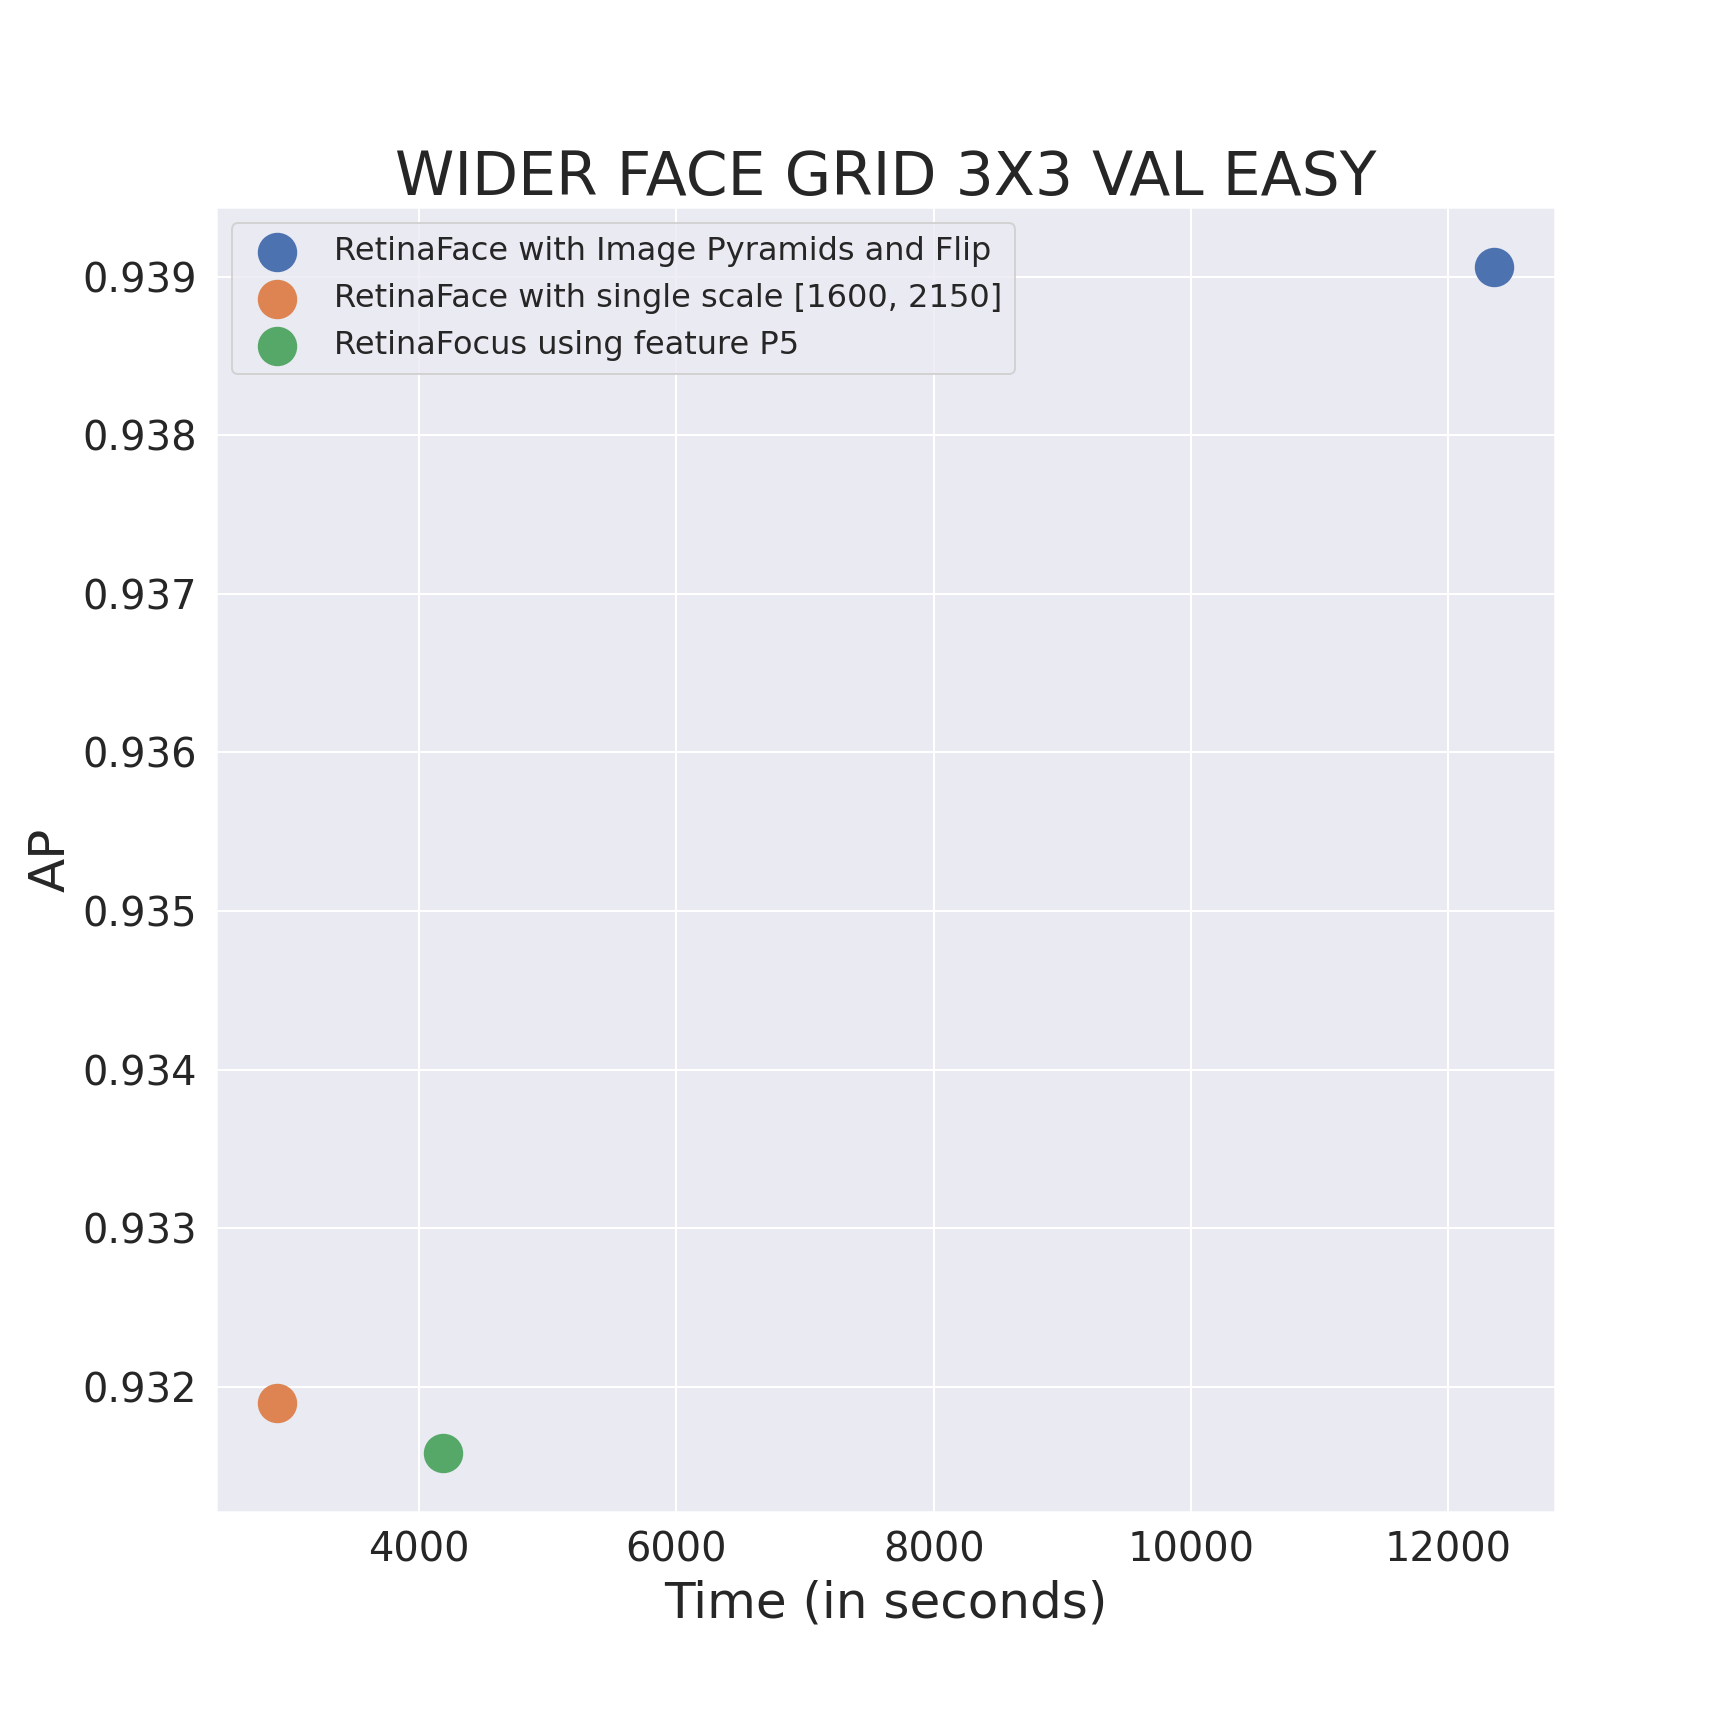
\includegraphics[width=7.3cm]{images/retinafocus_widerface_3k_val_easy_rtnf}} 
        \subfigure[]{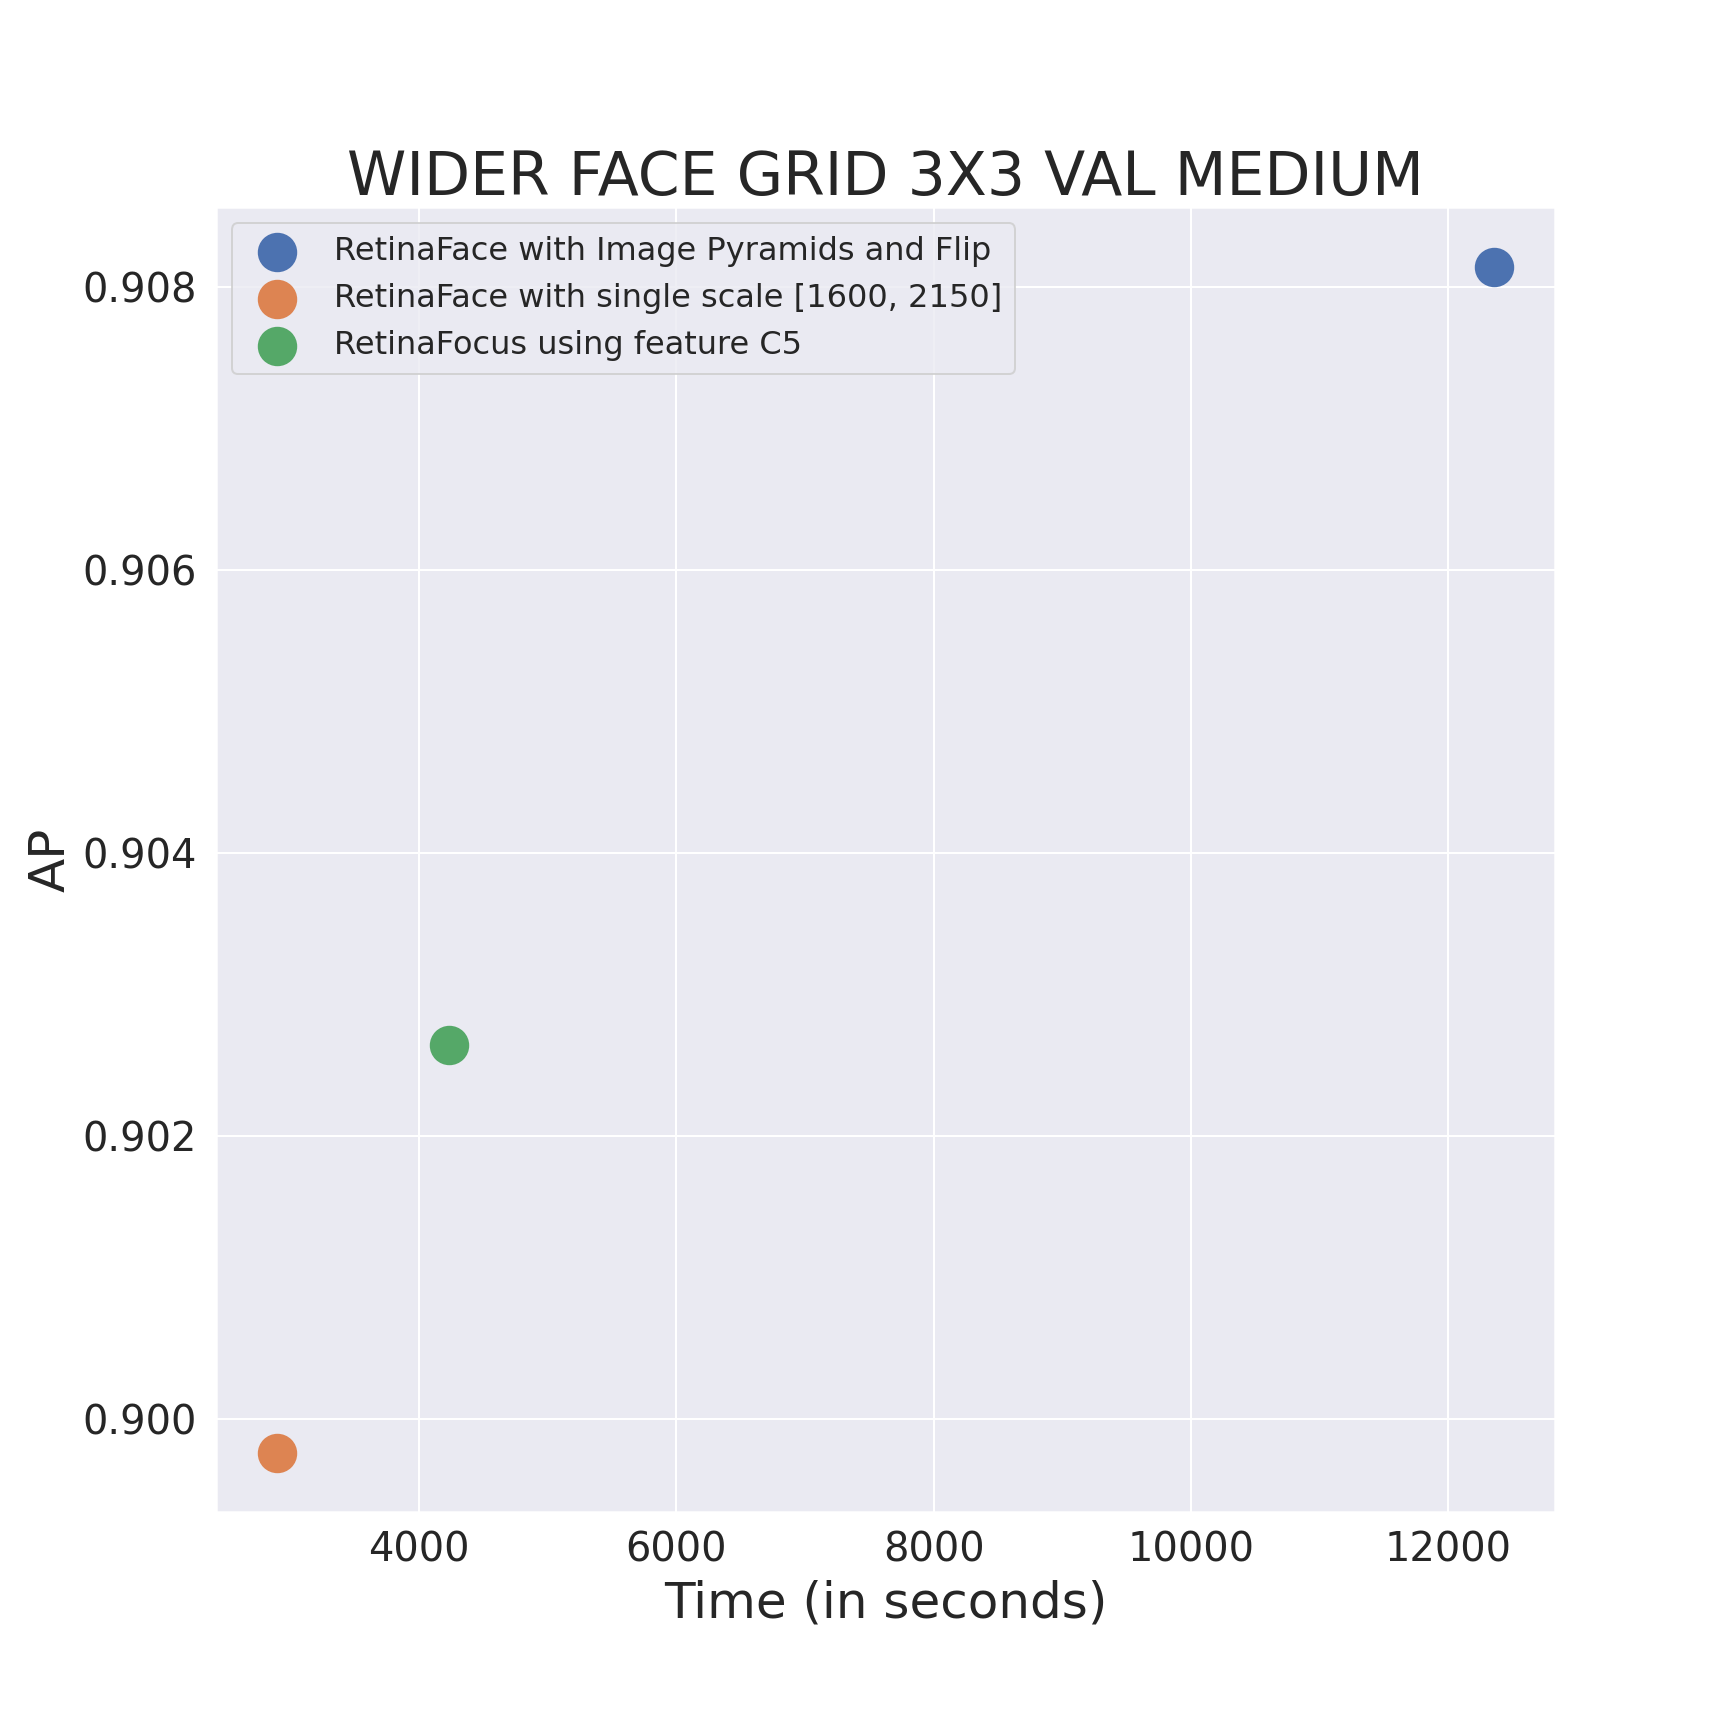
\includegraphics[width=7.3cm]{images/retinafocus_widerface_3k_val_medium_rtnf}} 
        \subfigure[]{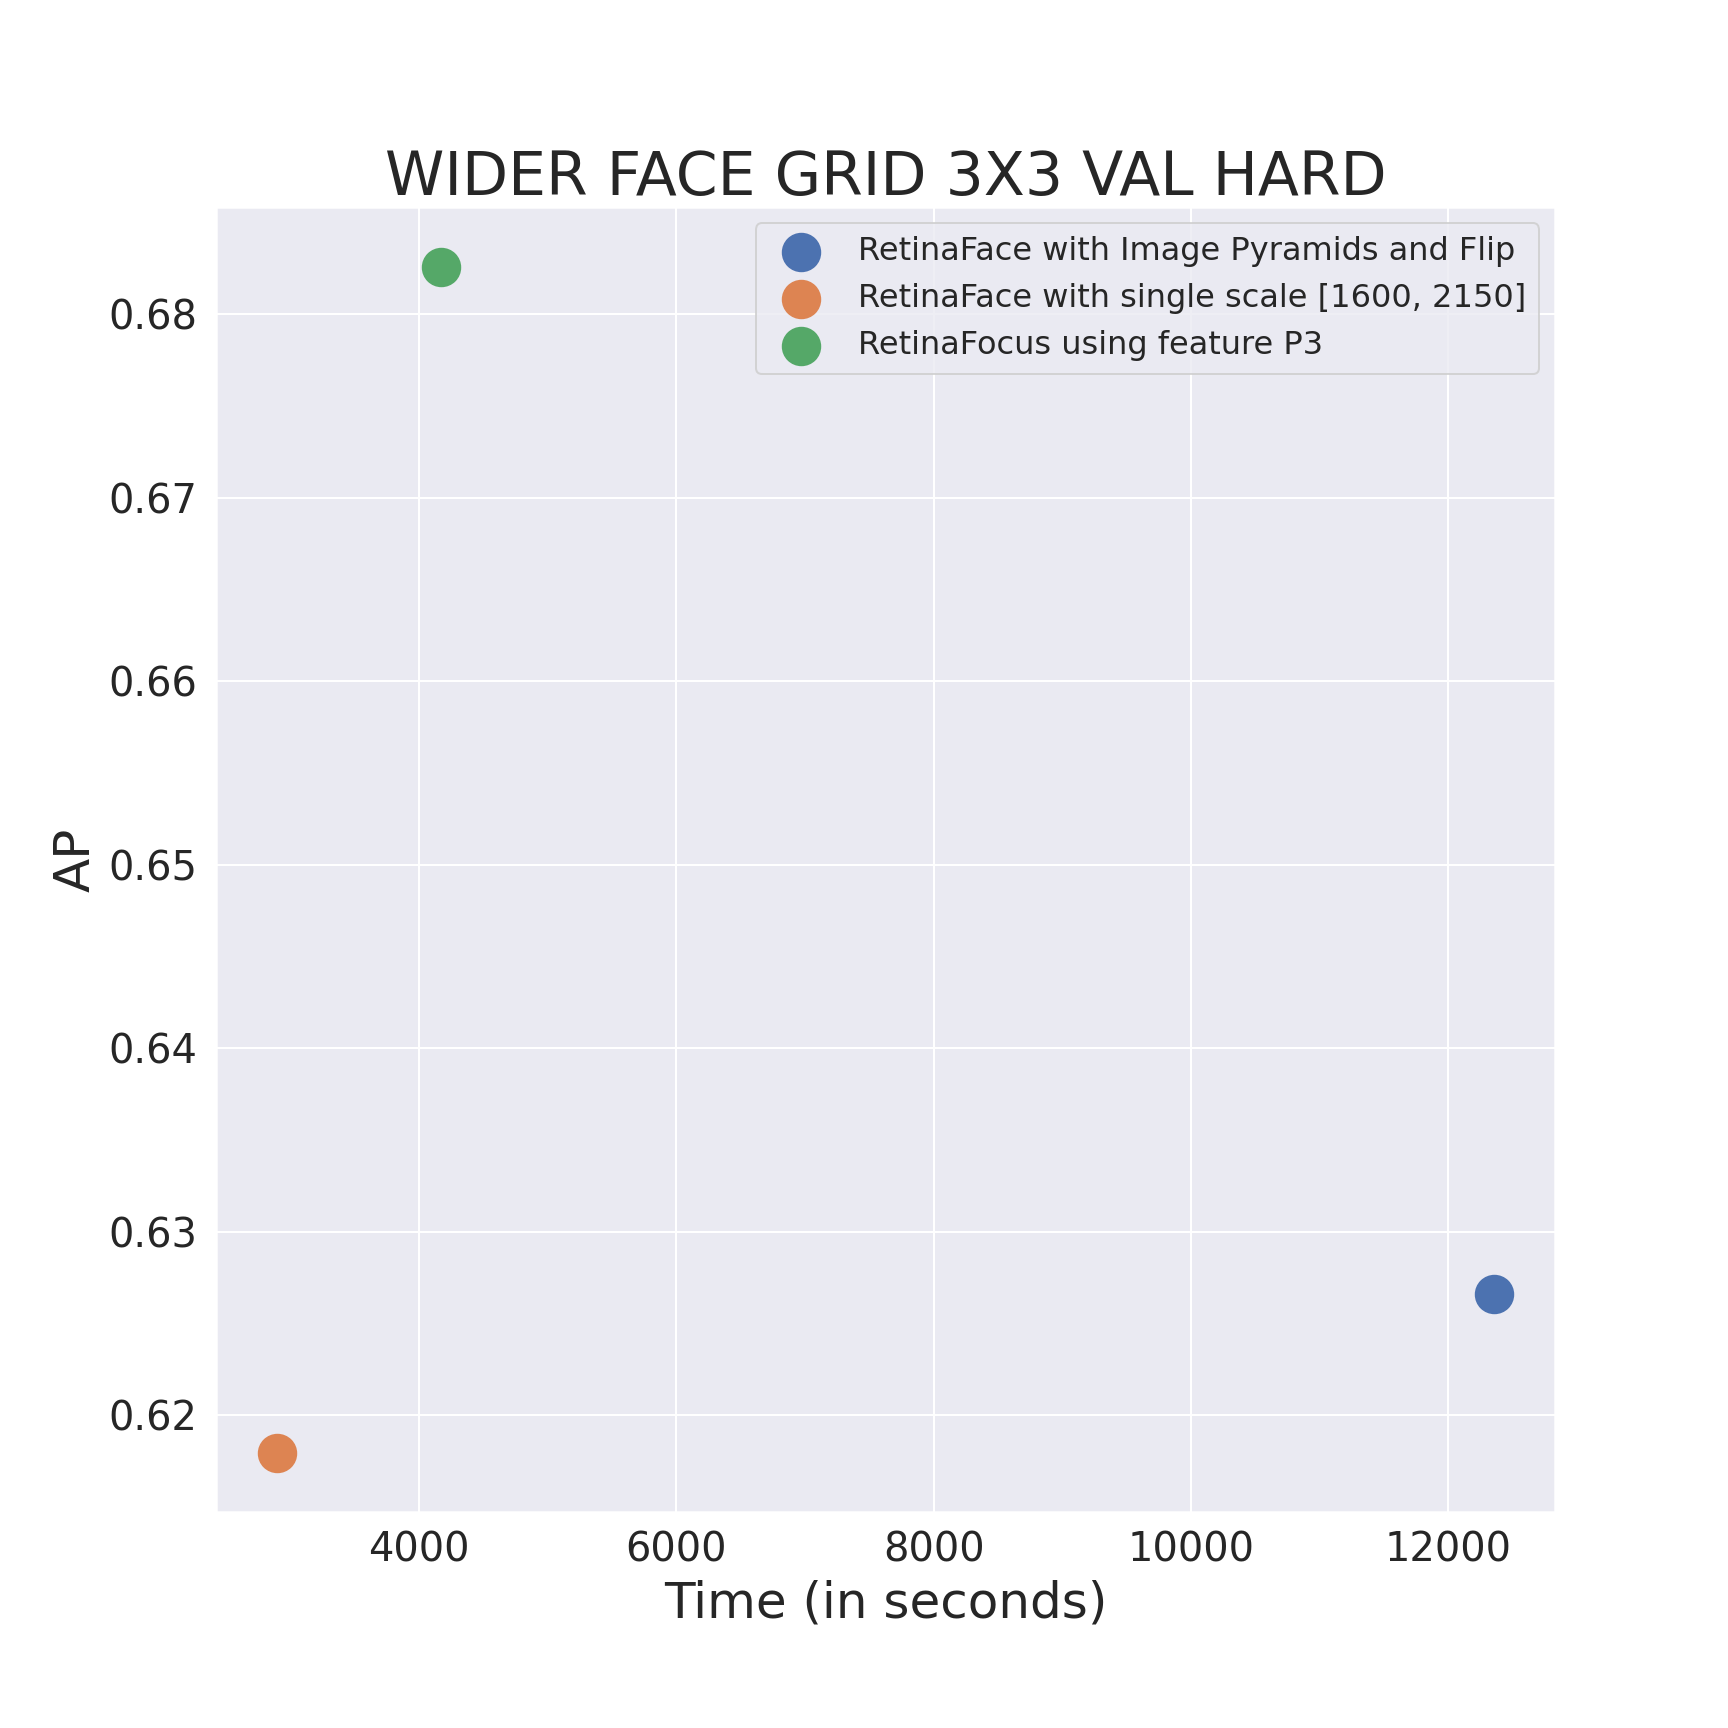
\includegraphics[width=7.3cm]{images/retinafocus_widerface_3k_val_hard_rtnf}} 
        \caption{Kết quả so sánh cấu hình tốt nhất của RetinaFocus với các cấu hình của RetinaFace trên ba bộ dữ liệu WIDER FACE kích thước lớn lưới $3 X 3$ val easy (a), medium (b) và hard (c)}
        \label{fig:retinafocus_widerface_3k_val_rtnf}
    \end{figure}
}